\documentclass[
    11pt,
    a4paper,
    egregdoesnotlikesansseriftitles,
    toc=chapterentrywithdots,
    openright,
    titlepage,
    parskip=half,
    headings=normal,  % reduces heading size
    listof=totoc,
    bibliography=totoc,
    index=totoc,
    captions=tableheading,  % caption below table
    chapterprefix,
    listof=flat,
    final,
    oneside,
    hyperref
]{scrbook}

\makeindex
% details about your thesis
\newcommand{\titel}{Analyse und Visualisierung von Datenqualität innerhalb eines Data Warehouse.}
\newcommand{\artderarbeit}{Bachelorarbeit}  % {Bachelorarbeit,Masterarbeit}
\newcommand{\autor}{Lukas Welsch}
\newcommand{\studiengang}{Informatik}  % {Informatik,Wirtschaftsinformatik,Medieninformatik}
\newcommand{\matrikelnr}{3201095}
\newcommand{\erstgutachter}{Prof.\,Dr.~Korbinian Riedhammer}
\newcommand{\zweitgutachter}{Prof.\,Dr.~Jens Albrecht}
\newcommand{\betreuer}{Dipl. Ing.\,~Andreas Sachs}
\newcommand{\unternehmen}{Sopra Financial Technology GmbH}
\newcommand{\logo}{figures/TH-Nuernberg-RGB.png}
\newcommand{\keywords}{hot, fuzz}
 

% custom head and foot
\usepackage[automark]{scrlayer-scrpage}
\pagestyle{scrheadings}
\ihead{\headmark}
\chead{}
\ohead{\pagemark}
\renewcommand*\chaptermarkformat{\chapappifchapterprefix{\ }% 
  \thechapter.\enskip}

\RedeclareSectionCommand[tocindent=0pt]{section}
\RedeclareSectionCommand[tocindent=0pt]{subsection}
%\RedeclareSectionCommand[tocnumwidth=70pt]{chapter}

\usepackage{scrhack}

% other packages
\usepackage[utf8]{inputenc}
\usepackage[T1]{fontenc}
\usepackage{lmodern,relsize,textcomp,csquotes}
\usepackage{amsmath,amsfonts}
\usepackage[english,ngerman]{babel}  % flip for German thesis
\usepackage[final]{graphicx}
\usepackage{setspace,geometry,xcolor}
\usepackage{makeidx}
\usepackage{paralist,ifthen,todonotes}
\usepackage{url}
\usepackage[toc]{glossaries}
\usepackage{pdfpages}

% table setup
\usepackage{longtable}
\usepackage{array}
\usepackage{ragged2e}
\usepackage{lscape}

% pdf hyperref
\usepackage[
    bookmarks=true,
    bookmarksopen=true,
    bookmarksnumbered=true,
    bookmarksopenlevel=1,
    pdftitle={\titel},
    pdfauthor={\autor},
    pdfcreator={\autor},
    pdfsubject={\titel},
    pdfkeywords={\keywords},
    pdfpagelabels=true,
    colorlinks=true,
    linkcolor=red,
    urlcolor=magenta,
    anchorcolor=black,
    citecolor=cyan,
    filecolor=magenta,
    menucolor=red,
    plainpages=false,
    hypertexnames=true,
    linktocpage=true,
]{hyperref}


% configure your listings style
\usepackage{listings}
\lstset{
	tabsize=3,
	extendedchars=true,
	frame=single,
	showstringspaces=true,
	numbers=left,
	numberstyle=\small,
	breakautoindent=true
}

% page setup
% \setlength{\topskip}{\ht\strutbox}
\geometry{paper=a4paper,left=2.5cm,top=3.0cm,bindingoffset=.8cm}
\onehalfspacing
\frenchspacing
\clubpenalty = 10000
\widowpenalty = 10000 
\displaywidowpenalty = 10000

% some commands
\newcommand{\ua}{\mbox{u.\,a.\ }}
\newcommand{\zB}{\mbox{z.\,B.\ }}
\newcommand{\dahe}{\mbox{d.\,h.,\ }}
\newcommand{\bzw}{\mbox{bzw.\ }}
\newcommand{\bzgl}{\mbox{bzgl.\ }}
\newcommand{\eg}{\mbox{e.\,g.\ }}
\newcommand{\ie}{\mbox{i.\,e.\ }}
\newcommand{\wrt}{\mbox{w.\,r.\,t.\ }}
\newcommand{\etal}{\mbox{\emph{et.\,al.\ }}}


% TODO remove if not needed...
\usepackage{blindtext}

% load glossary entries
\makenoidxglossaries
\loadglsentries{glossary}

\begin{document}
\selectlanguage{ngerman}

\setcounter{secnumdepth}{3}  % numerate subsections
\setcounter{tocdepth}{2}  % ...but don't include them in toc

\frontmatter
\thispagestyle{empty}
\pdfbookmark[1]{Cover}{cov}
\begin{titlepage}

\begin{center}

%\includegraphics[width=\linewidth]{figures/TH-Nuernberg-RGB.png}\\[1cm]
\LARGE{Fakultät Informatik}\\[2cm]

\huge
\textbf{\titel}\\[1cm]
%
\Large
\artderarbeit~im Studiengang \studiengang\\[1cm]
%
\large
vorgelegt von

\Large
\autor\\[0.5cm]
\small
Matrikelnummer \matrikelnr\\[2cm]

\vspace*{\fill}

\large
\begin{tabular}{p{3cm}p{8cm}}\\
Erstgutachter:  & \quad \erstgutachter\\[1.2ex]
Zweitgutachter: & \quad \zweitgutachter\\[1.2ex]
%discomment "Betreuer" and "Unternehmen" for a thesis in a company
Betreuer: & \quad \betreuer\\
Unternehmen: & \quad \unternehmen
\end{tabular}
\end{center}

\begin{center}
\copyright\,\the\year
\end{center}

\vspace{-0.5cm}
\singlespacing
\small
\noindent Dieses Werk einschließlich seiner Teile ist \textbf{urheberrechtlich geschützt}.
Jede Verwertung außerhalb der engen Grenzen des Urheberrechtgesetzes ist ohne Zustimmung des Autors unzulässig und strafbar.
Das gilt insbesondere für Vervielfältigungen, Übersetzungen, Mikroverfilmungen sowie die Einspeicherung und Verarbeitung in elektronischen Systemen.

\end{titlepage}
\cleardoublepage

% download the following form and complete it (hit save in your editor)
% https://intern.ohmportal.de/fileadmin/Gelenkte_Doks/Abt/SZS/SB/SB_0050_FO_Pruefungsrechtliche_Erklaerung_und_Erklaerung_zur_Veroeffentlichung_der_Abschlussarbeit_public.pdf
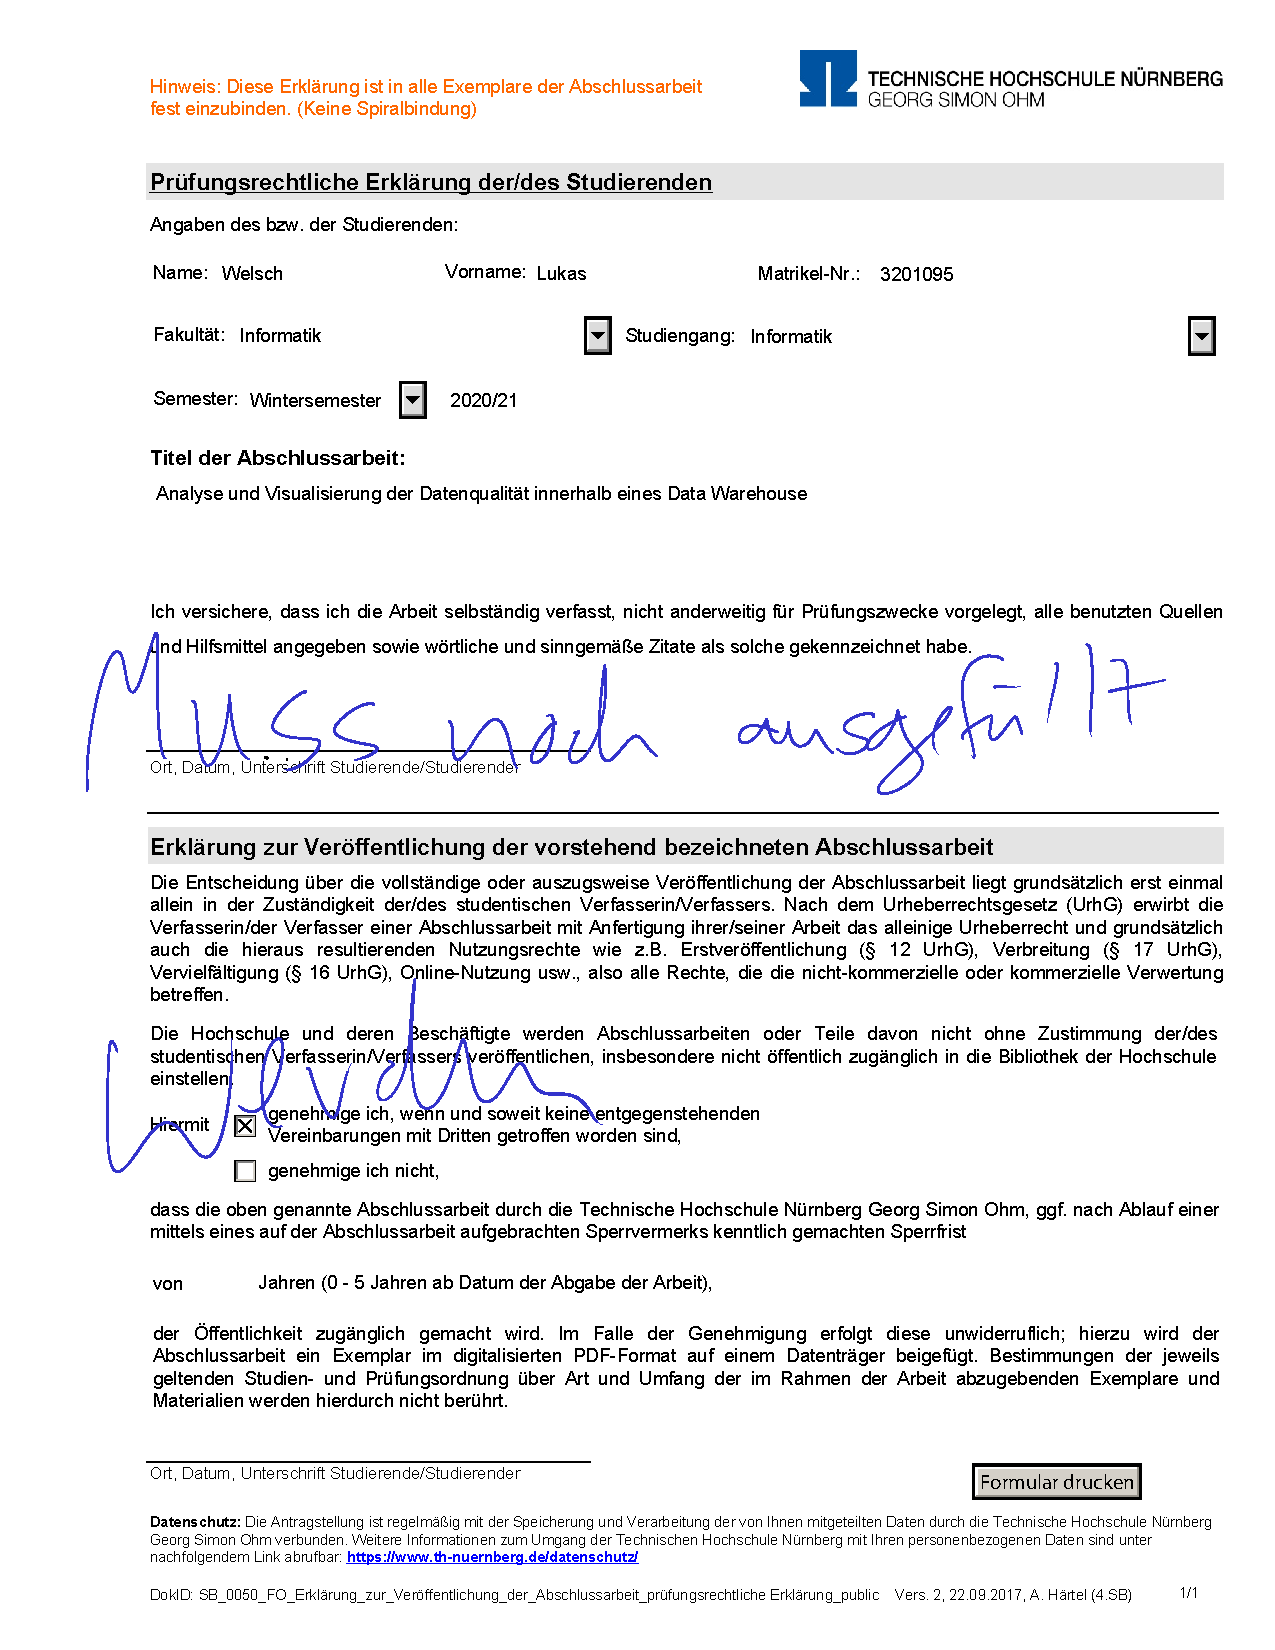
\includepdf{SB_0050_FO_Pruefungsrechtliche_Erklaerung_und_Erklaerung_zur_Veroeffentlichung_der_Abschlussarbeit_public.pdf}\cleardoublepage

\thispagestyle{empty}
\section*{Kurzdarstellung}
\label{sec:kurzdarstellung}
Kurze Zusammenfassung der Arbeit, höchstens halbe Seite.
Deutsche Fassung auch nötig, wenn die Arbeit auf Englisch angefertigt wird.

\blindtext


\section*{Abstract}
\label{sec:abstract}
\emph{Only if thesis is written in English.}

\blindtext
\cleardoublepage

\tableofcontents

\mainmatter
\chapter{Einleitung}\label{ch:intro}

%You may have read about similar things in \cite{Goodliffe2007}.
%You can also write footnotes.\footnote{Footnotes will be positioned automatically.}
%It is possible to reference glossary entries as \gls{library} as an example.




- Kann mit Hilfe von ML-Verfahren berechnet werden, ob Risikobewertungen über Kunden aktualisiert werden müssen? 
% externe Dienstleister bündeln die Informationen mehrerer Kreditvergeber. 
% Deshalb werden die Daten von dort vermutlich immer akurater sein und können nicht ersetzt werden
- Können die vorliegenden MetaDaten visualisiert werden, sodass Erkenntnisse zur (Prozess)-Qualität gewonnen werden können? 

\cite{d.kelleher2015a}
\cite{d.kelleher2015}

%IDEEN
%versch. Arten visualisieren und dann selbst entscheiden bzw Entscheidungen von Experten mit einfließen lassen
%Anpassung der Adressen aus den letzten Jahren (Durchschnitt wie oft wird Kundenstammdaten aktualisiert)



% Problematisch ist, dass die IT-Systeme so gestaltet sind, dass diese Freitextfelder verfügbar sind, sodass erst keine Rechtschreibfehler entstehen können. 
% Allerdings steht die Bank vor dem Problem die Daten schon erhoben zu haben und benötigt jetzt eine Lösung, um diese auszubessern. 


\chapter{Grundlagen}\label{ch:data}

\section{Definition von Datenqualität}
Datenqualität wird in der Literatur auf verschiedene Arten definiert. 
Viele Datenqualitätsstudien verwenden Korrektheit als einziges Datenqualitätsmerkmal. \cite{wang1996}
Datenqualität umfasst jedoch nicht nur die Korrektheit von Daten, sondern auch anderen Dimensionen. 
Ein Paper von Oliva, Zubcoff und Mazón zeigt den Einfluss von anderen Dimensionen, wie zb. Vollständigkeit auf die Erkennungsrate von Klassifikatoren \cite{espinosaoliva2011} Die Autoren schlagen vor den Aufbereitungsprozess und vor allem Datenqualität nicht nur auf die Korrektheit von Daten zu beziehen sondern auch auf die anderen Datenqualitätsdimensionen zu achten.

\subsection{Datenqualitätsdimensionen}
Die Dimensionen Richtigkeit, Vollständigkeit, Konsistenz und Aktualität werden in den meisten Veröffentlichungen genannt, allerdings gibt es keinen Standard, weder im Bezug auf die verwendeten Dimensionen, noch die Definition der Dimensionen. \cite{scannapieco2002}
Da keine allgemeine Empfehlung zur Verwendung von Dimensionen existiert werden in dieser Arbeit die Datenqualitätsdimensionen verwendet, die in den meisten Veröffentlichungen auftauchen.
Dies kann dem Paper von Scannapieco und Catarci entnommen werden. 
Diese Dimensionen sind für die Auswertung der Methoden im Rahmen der Arbeit geeignet. 
Jede dieser Datenqualitätsdimensionen umfasst eine Facette der Datenqualität und werden im Folgenden nach Wand und Wang beschrieben \cite{wand1996}. \\

\textbf{Richtigkeit} \\
Richtigkeit wird als Gleichheit zwischen zwei Werten definiert, sodass die Daten die Wirklichkeit korrekt repräsentieren. 
Beispiel: Eine Person mit dem Namen Max Mustermann ist als Mx Mustermann abgespeichert. 
Die gespeicherten Daten repräsentieren nicht die Wirklichkeit, sie sind somit nicht richtig. \\

\textbf{Aktualität / temporäre Richtigkeit} \\
Als Spezialisierung der Richtigkeit kann die temporäre Richtigkeit gesehen werden, die richtige Repräsentation zu einem bestimmten Zeitpunkt oder Zeitspanne beschreibt. 
Die temporäre Richtigkeit zum aktuellen Zeitpunkt wird auch als Aktualität bezeichnet. \\

\textbf{Vollständigkeit} \\
Die Daten sind umfangreich genug für die jeweilige Aufgabe. \cite{wang1996} 
Da ein Data Warehouse aus relationalen Datenbanken besteht, wird die Vollständigkeit im Folgenden auf relationale Datenbanken bezogen.
Die Vollständigkeit wird von \cite{pipino2002} in drei Klassen kategorisiert.
\begin{itemize}
 \item Schema: Grad der Daten, die nicht im Schema fehlen
 \item Spalte: Anzahl der fehlenden Werte innerhalb einer Spalte
 \item Population: Wenn eine Spalte alle 16 Bundesländer beinhalten sollte, aber nur 14 vorhanden sind, dann herrscht Populationsunvollständigkeit \\
\end{itemize} 

\textbf{Konsistenz} \\
Die gleichen (redundanten) Datensätze haben die gleichen Werte in verschiedenen Tabellen. 
Ein Beispiel für Konsistenz ist die referentielle Integrität, die sicherstellt, dass Datensätze nur auf existierende Datensätze verweisen. 
\\ % \textbf{Appropriate Amount of Data, Believability, }

Für diese Arbeit stehen die Dimensionen Richtigkeit, Aktualität und Vollständigkeit im Vordergrund. 
Dies liegt daran, dass eine Konsistenzprüfung von einem Datenbanksystem automatisch vorgenommen wird. 
Es ist deshalb bei relationalen Daten in der dritten Normalform nicht notwendig diese auf die Konsistenz zu prüfen, da durch die Verwendung der Normalform Redundanzen ausgeschlossen werden. % TODO Quelle Finden!
In einem Data Warehouse werden Daten hingegen in sogenannten Data Marts redundant gespeichert, um eine höhere Leseperformance für die einzelnen Endanwendungen bieten zu können. %TODO Kapitel Alternative DW/BI Architectures
Allerdings können Probleme, die durch Data Marts entstehen einfach mit einer richtigen Modellierung behoben werden. \cite{kimball2002}

In dem vorliegendem Data Warehouse existiert eine Data Vault Architektur. 
In dieser werden die Daten aus Performancegründen redundant abgespeichert. 
Deshalb kann es zu Inkonsistenzen im Datensatz führen. \cite{bolt2020}
Hierfür existiert bereits eine Methode in der Data Warehouse Abteilung.
Dabei werden die Daten zusammengeführt und überprüft, ob Datensätze mit dem gleichen Schlüssel unterschiedliche Werte besitzen. 
Obwohl dieses Szenario in der Realität selten eintritt, ist eine solche Prüfung für die Inkonsistenzvermeidung signifikant. 

\subsection{Metriken der Dimensionen}
Um diese eher abstrakten Definitionen messbar zu machen haben sich einige Verfahren etabliert.
Diese lassen sich grob in die Kategorien subjektiv und objektiv aufteilen, vgl. \autoref{fig:subjektiv} nach Pipino. 


Bei den subjektiven Verfahren wird die vorherrschende Datenqualität durch Experten geschätzt. 
%Dieses Verfahren ist allerdings nicht nur zeitaufwendig für die Experten, sondern ist auch fehleranfällig. \textcolor{red}{\textbf{HIERZITATANGEBEN}} \cite{}
Eine weitere Möglichkeit besteht darin objektive Verfahren zu verwenden, bei denen mit Hilfe von mathematischen Funktionen die Datenqualität berechnet oder geschätzt wird. 

Des weiteren gibt es ein kombiniertes Verfahren, bei dem Grenzwerte von Experten geschätzt und anschließend durch mathematische Funktionen abgeglichen werden. 
Das kombinierte Verfahren kann durch Quadrate visualisiert werden, die an der y-Achse die subjektive Bewertung und auf der x-Achse die objektive Bewertung zeigen, vgl. \autoref{fig:subjektiv}. 
Diese sind aufgeteilt in hohe bzw. niedrige Datenqualität.
Ziel einer Datenqualitätsmaßnahme ist es sowohl eine hohe subjektive als auch hohe objektive Datenqualität zu erlangen.
Bei einer guten Datenqualität liegt das Ergebnis im IV. Quadrant. \cite{pipino2002} 


\begin{figure}[hbt!]
\centering
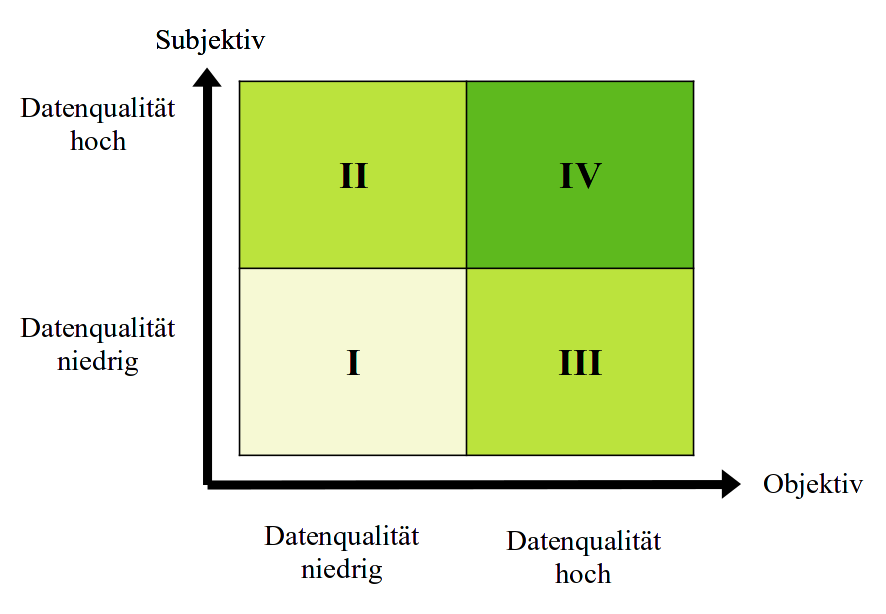
\includegraphics[width=100mm,scale=1]{content/subjektiv_objektiv.png}
\caption{Eigene Darstellung der Auswertung von objektiven und subjektiven Verfahren, basiert auf der Abbildung von \cite{pipino2002}}\label{fig:subjektiv}
\end{figure}




\section{Standardisierter Prozess}
Der Erfolg von Projekten kann durch die Verwendung eines standardisierten Prozesses deutlich gesteigert werden.
Einer der für Data Mining Projekte am weitesten verbreitet und eingesetzte Prozess ist der Cross Industry Standard Process for Data Mining (CRISP-DM). \cite{d.kelleher2015crispdm}
Der Prozess beinhaltet die Phasen, die nötig sind, um ein Data Mining Projekt durchzuführen. 
Des weiteren ist definiert, welche Aufgaben in der jeweiligen Phase anfallen und welche Ergebnisse die Phasen hervorbringen \cite{wirth2000}.

\begin{figure}[h]
\centering
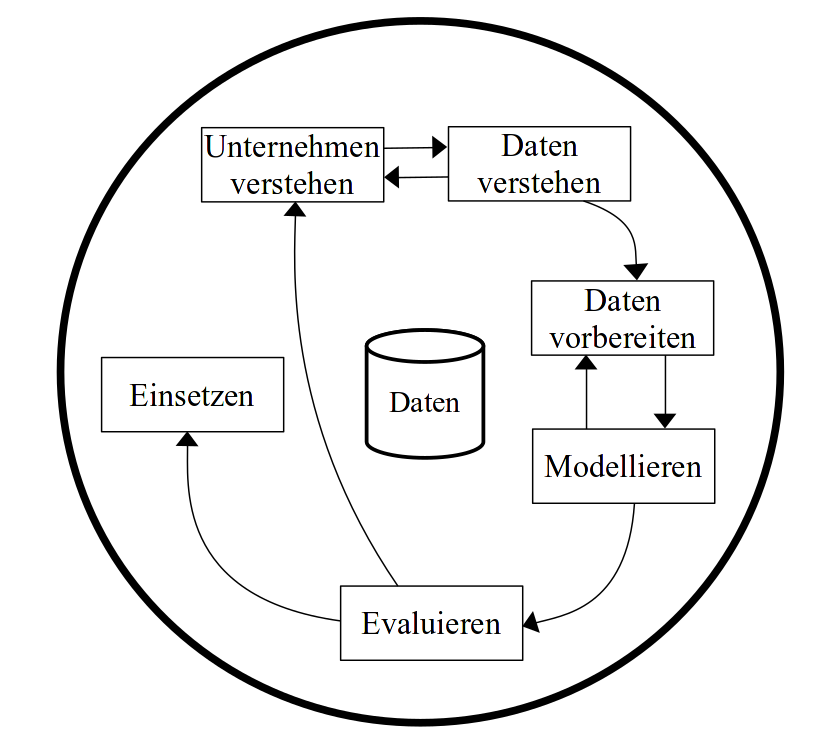
\includegraphics[width=100mm,scale=1]{content/CRISP-Prozess.png}
\caption{Eigene Darstellung des CRISP-DM, basiert auf der Abbildung von \cite{wirth2000}}\label{fig:crisp}
\end{figure}
In der \autoref{fig:crisp} sind die Phasen und ihre Ablaufreihenfolge zu sehen. 
In der Grafik ist zu erkennen, dass es sich bei dem CRISP-DM um einen iterativen Prozess handelt.
Auch in dieser Bachelorarbeit wird nach diesem Vorgehensmodell gearbeitet. 
Die Bestandteile des Modells finden sich in den einzelnen Kapiteln wieder. 
Für die Visualisierung und das Erstellen des Dashboards wird die Phase Modellieren durch Visualisieren ersetzt. 
\\

Die Bestandteile des Prozesses sind: \\
\begin{enumerate}
 \item \textbf{Unternehmen verstehen} \\
 Bei diesem Punkt ist die Aufgabe herauszufinden, welches Problem das Unternehmen versucht zu lösen \cite{d.kelleher2015crispdm}.
 
 Das Verständnis für das Problem des Unternehmens wird in dieser Bachelorarbeit in \autoref{ch:anforderungen} mit Hilfe einer Stakeholder-Analyse erlangt. Hierbei werden die betroffenen Personen untersucht und deren Wünsche aufgezeigt. Als Ergebnis werden drei mögliche Verfahren skizziert, die anschließend genauer erläutert werden.  
 
 \item \textbf{Daten verstehen} \\
 Um die Probleme mit Hilfe von Daten lösen zu können, müssen die vorhandenen Daten genau verstanden werden. Es ist wichtig zu verstehen, welche Daten in welcher Quelle vorhanden sind und um welche Datenarten es sich handelt. \cite{d.kelleher2015crispdm} 
 
 Diese Phase ist in \autoref{ch:data} umgesetzt. Dort werden die einzelnen Quellen untersucht und die Ausprägungen der Datenattribute analysiert. Des weiteren werden in dieser Phase die für die Lösung des skizzierten Problems die relevanten Daten aus den Quelltabellen ausgewählt. 
 
 \item \textbf{Daten vorbereiten} \\
 In dieser Phase wird die finale Tabelle aus den Quellen konstruiert, die zum Training der ML-Modelle verwendet wird. Typische Aufgaben in dieser Phase sind die Attributauswahl, Datenbereinigung und das Erzeugen von neuen Eigenschaften anhand der bestehenden Daten. \cite{wirth2000} Diese Tabelle wird auch als Analytical Base Table (ABT) bezeichnet \cite{d.kelleher2015crispdm}.
 
 Die Datenvorbereitung geschieht an zwei Stellen in dieser Bachelorarbeit. 
 Die Konstruktion der ABT geschieht in dem \autoref{ch:data} und die Datenbereinigung wird im \autoref{ch:experiments} durchgeführt. %TODO Lieber auch in dem Kapitel Daten mitmachen? 
 
 \item \textbf{Modellieren} \\
 In dieser Phase werden verschiedene ML-Modelle ausgewählt und getestet.
 Die Modellierungsphase ist stark verbunden mit der Datenvorbereitung, da sich einige Probleme in den Daten erst erkennen lassen, wenn die Modelle angewendet werden. 
 Auch neue Ideen für die Konstruktion von Merkmalen anhand der bestehenden Daten kann in dieser Phase gefunden werden. \cite{wirth2000}
 
 Die Modellierung und das Testen verschiedener Ansätze ist in dem \autoref{sub:machine_learning} zu sehen. 
 Zur Umsetzung der Visualisierung wird an dieser Stelle kein Modell ausgewählt und getestet, sondern die verschiedenen Data Quality Dashboard Tools untersucht. 
 Des Weiteren wird in dieser Phase die Visualisierungen in dem evaluiertem Tool erzeugt und die Ergebnisse präsentiert. 
 
 \item \textbf{Evaluieren} \\
 An dieser Stelle im Prozess wird nochmals überprüft, ob das Modell die Probleme, die in Phase 1 analysiert wurden, behebt.
 Das Hauptziel ist herauszufinden, ob ein Unternehmensziel nicht gut genug durchdacht wurde. \cite{wirth2000}
 Es wird außerdem evaluiert, ob die das trainierte Modell für den Einsatzzweck geeignet ist und nicht von Over- bzw. Underfitting geprägt ist. \cite{d.kelleher2015crispdm}
 
 Die Evaluation der Machine Learning Modelle erfolgt in \autoref{sub:evaluation}. 
 Dort werden die üblichen Metriken verwendet, um die Modelle zu testen und miteinander zu vergleichen. 
 
 Zur Auswertung der Visualisierung werden die gestellten Anforderungen, die in der Stakeholder-Analyse erhoben werden, mit den Ergebnissen verglichen. 
 Dies erfolgt in \autoref{sub:visualisierung}.
 
 \item \textbf{Einsetzen} \\
 Als Abschluss des Prozesses steht die Verwendung des Datenprojektes in einer produktiven Anwendung \cite{d.kelleher2015crispdm}.
 Hierzu zählt die Integration des Datenprojektes in das Unternehmen und dessen IT-Prozessen. 
 Oft wird dieser Part nicht mehr von dem Datenanalysten durchgeführt, sondern von dem Unternehmen selbst.
 Wichtig ist hierbei, dass die Schritte klar sind, was zu tun ist, um die Anwendung bzw. das ML-Modell nutzbar zu machen. \cite{wirth2000}
 
 
 %TODO Neues Unterkapitel in Experimente, dass die Integration grob beschreibt oder in den Aublick?
 Auch in dieser Arbeit werden die Schritte beschrieben, die nach dem Projekt nötig sind. 
 In großen Teilen werden diese auch schon implementiert und durchgeführt. 
 Lediglich das automatisierte Starten der Programme muss durch die Entwicklungsabteilung hinzugefügt werden, da diese es in ihrer Programmsteuerung hinterlegen können. 
 In diesem Projekt wird eine solche Steuerung beispielhaft mit der Verwendung von CRON-Jobs beschrieben. 
\end{enumerate}





\chapter{Anforderungsanalyse}\label{ch:anforderungen}
Um aus dem Data Warehouse die geeigneten Daten zu extrahieren und Methoden zur Analyse und Visualisierung der Datenqualität auszuwählen, ist es zunächst notwendig eine Stakeholder-Analyse durchzuführen. 
Auf Basis dieser Analyse ist es anschließen möglich die relevanten Daten aus dem Data Warehouse zu ermitteln, die für die Durchführung der Methoden notwendig sind. 



Für eine Datenqualität, die sich in einem Unternehmen etablieren kann, ist es nötig diese von den Gesichtspunkten aller Stakeholdern zu betrachten.
Anhand einer Stakeholder-Analyse wird es möglich sein die Probleme der Datenqualität auf zwei Ebenen zu betrachten. 
Zum einen benötigen die Business-User gute Datenqualität, um die richtigen Zinsen anhand des Risikoscorings zu vergeben und auf der anderen Seite benötigen die Entwickler eine Möglichkeit, um ihre ETL-Strecken zu überprüfen.
Für diese beiden Probleme können zwei verschiedene Verfahren eingesetzt werden.
Zur Identifikation und Überprüfung des Risikoscores kann ein Machine Learning Algorithmus trainiert werden, der die korrekten Werte vorhersagt und somit einen Aufschluss darüber gibt, wie viele Datensätze aktualisiert werden sollten.
Um die ETL-Strecken zu analysieren sind die Metadaten zu den Prozessen nötig, die anzeigen, wie viele Daten an jedem Tag extrahiert wurden. 
Auffälligkeiten können dann genutzt werden, um Maßnahmen einzuleiten.
Hierfür bietet sich eine Visualisierung an, die in Echtzeit die Daten verarbeitet, analysiert und anschließend interpretierbar darstellt.
Die beiden beschriebenen Verfahren werden in dem Kapitel Experimente durchgeführt. 
%Datakitchen



\section{Stakeholder-Analyse}
\label{sec:Stakeholder-Analyse} 
Mit Hilfe einer Stakeholder-Analyse ist es möglich, die negativen Einflüsse zu erkennen und die positiven Einflüsse zu nutzen.
Zum Anderen können die Erwartungen der einzelnen Stakeholder erkannt und die Projektziele richtig gewichtet werden. \\
Die Stakeholder-Analyse wird nach folgenden Schritten durchgeführt: 

\begin{enumerate}
 \item Stakeholder identifizieren
 \item Stakeholder Einfluss analysieren
 \item Aktionsplanung (Maßnahmen ableiten)
\end{enumerate} \cite{salzsearch}

% Nach \cite{pipino2002} gibt es drei Stakeholder: the collector (Sammler) , custodians (Verwalter) and consumers (Verbraucher) of data products.  

\subsection{Stakeholder identifizieren}
In diesem Schritt werden die Stakeholder genannt, kurz beschrieben und visualisiert. 
Aufgrund der Analyse des mittelständischen Unternehmens aus der Bankenbranche können folgende Stakeholder identifiziert werden: Entwickler, Business User und Bankmitarbeiter.
Diese werden im Folgenden genauer analysiert und beschrieben. 


\begin{itemize}
% \itemsep-2em 
\item \textbf{Entwickler} \\            
Als Stakeholder lassen sich zunächst die Entwickler identifizieren.
Diese sind für die Einhaltung einer guten Datenqualität unmittelbar wichtig, da diese die Extraktionsprozesse entwickeln, die zu Fehlern in der Datenqualität führen können.
%Warum kann es überhaupt passieren, dass nicht alle Daten exportiert werden?
Die Daten werden von einem legacy-System in das Data Warehouse übertragen, indem die Daten aus einer hierarchischen Datenbank als Datei abgelegt werden.
Ein Prozess iteriert über alle Dateien und extrahiert die Daten, die anschließend neu strukturiert im Data Warehouse abgelegt werden.
Aufgrund von einigen Problemen in der Extraktion kann es dazu führen, dass die Daten nicht korrekt extrahiert werden.
Für diesen Fall gibt es eine Überwachung der Programme, die einen Fehler bei der Verarbeitung meldet.
Wenn jedoch weniger oder mehr Daten verarbeitet werden als üblich deutet dies auch auf einen Fehler in der Extraktion hin. 
Dieser Fall wird aktuell noch durch keinen Mechanismus oder Programm erkannt. 
Als Lösung für dieses Problem bietet sich eine Visualisierung an, anhand der die Schwankungen aufgezeigt und dargestellt werden können. 
Ein Entwickler kann anhand der Visualisierung erkennen, ob durch seine Programmänderung die Schwankung der Datenmengen innerhalb der saisonalen Schwankungen ist oder, ob seine Änderung einen neuen Fehler verursacht hat. 
%Probleme: Keine Datei wird mehr an einem Ordner abgelegt, weil fehler im anderen System -> keiner merkt was, Daten nicht mehr aktuell
%Probleme: Zweite Änderung während Extraktion läuft -> Primärschlüssel doppelt -> deduplizierung -> wenn fehler in Primkey, dann werden ganz viele Daten gelöscht, was ungewöhnlich ist
%Allerdings werden die Dateien teilweise nicht schnell genug abgeholt und die Daten werden überschrieben


\item \textbf{Business User}       \\
Auf der anderen Seite gibt es die Business User, die beispielsweise die Gesamtbanksteuerung übernehmen.
Bei diesem Teilgebiet wird errechnet, wie gut die Zinssätze sein dürfen, sodass die Bank Gewinn erzielt und gleichzeitig möglichst viele Kunden zufrieden stellen kann.
Für diesen Stakeholder sind alle Dimensionen wichtig, da nur mit einer sehr guten Datenqualität eine optimale Gesamtbanksteuerung vorgenommen werden kann. 
Würde der Stakeholder nur über falsche, unvollständige und veraltete Daten verfügen, könnte dies Verluste für die Bank zur Folge haben.
Besonders entscheidend ist für diesen Stakeholder, dass der Wert für den Risikoscore richtig und aktuell ist.
Beim Risikoscoring werden die Daten der Kunden an einen externen Dienstleister gesendet.
Dieser berechnet einen Risikoscore, anhand dessen die Zinsvergabe erfolgt.
%CRM sind auch Business User, die korrekte Daten haben wollen

\item \textbf{Bankmitarbeiter}      \\
Des weiteren ist der Bankmitarbeiter Bestandteil der Kreditvergabe. 
Die Kreditvergabe erfolgt anhand einer Bewertung des Kunden, je nachdem wie gut der Risikoscore des Kunden ist, umso bessere Zinssätze erhält dieser.
Für den Bankmitarbeiter ist es wichtig, dass die Daten zum Risikoscoring sowohl richtig als auch aktuell sind.

\end{itemize}




Nicht nur Fehler in numerischen Daten, sondern auch in Texten sind festzustellen. 
Dies führt zu falschen Interpretationen bzw. dazu, dass ein Kunde nicht den richtigen Risikoscore erhält. 
Auch fehlende Daten führen zu Fehlern.
Dies ist ein Fall, der sowohl für den Kunden als auch für die Bank selbst zu einem Problem führt. 
Der Kunde erhält nicht den für ihn bestmöglichen Risikoscore und die Bank verliert einen Kunden, da diese verglichen mit der Konkurrenz nicht den besten Kredit vergeben kann. 
Es kann allerdings auch passieren, dass die Bank dem Kunden einen besseren Score vergibt, da der Beruf falsch interpretiert wird und muss somit ein höheres Risiko eingehen und die Bank kann ihr Risiko nicht korrekt abschätzen. 






Die beschriebenen Stakeholder werden mit ihren Erwartungen an das Projekt in der folgenden Grafik dargestellt.
\subsection{Betroffenheitsanalyse}
\begin{tabular}[h]{l|p{2cm}|>{\centering}p{1.5cm}|p{2.5cm}|c|c|p{3cm}}
ID & Wer        & Betroffen-heit & Erwartung & Macht & Einstellung & Maßnahmen  \\ \hline
S1 & Entwickler & m             & Fehler in der Entwicklung werden angezeigt; Wenig Programmieraufwand & g & Neutral & Erklärung der Notwendigkeit, Zeitvorteil aufzeigen  \\ \hline
S2 & Business User & h          & Daten sollten fehlerfrei und aktuell sein & g & Positiv & - \\ \hline
S3 & Bank-mitarbeiter & h          & Daten müssen immer verfügbar und richtig sein & h & Positiv & - \\
\end{tabular}


Welchen Stakeholder interessiert welche Dimension?

\begin{tabular}[h]{l|l|l}
Stakeholder & Dimension & Begründung \\ \hline
Entwickler & Vollständigkeit & Der Entwickler geht davon aus, dass die Daten die vom Quellsystem abgeholt werden richtig sind. Für ihn ist deshalb die Dimension Vollständigkeit interessant, da er wissen muss, ob die richtige Anzahl an Daten exportiert wurden. \\ \hline
Business User & Alle Dimensionen & \\ \hline
Bankmitarbeiter & Keine Dimension & Geht davon aus, dass die Datenqualität schon geprüft wurde \\
\end{tabular}


Für Welche Stakeholder kann sollte welches Verfahren angewendet werden?
- Business User: Risikoscoring sollte immer aktuell sein, dabei kann ein ML Verfahren verwendet werden, um die Daten zu klassifizieren und bei großer Abweichung können diese Daten dann aktualisiert oder neu angefordert werden.

- Bank Mitarbeiter: ?
- 

In dieser Bachelorarbeit wird die Verwendung von Machine Learning Verfahren zur Verbesserung der Datenqualität untersucht.
Deshalb bietet sich das Thema Risikoscoring am besten an, da es feste Ausgangswerte (Labels) bietet, die trainiert werden können.
Der trainierte Klassifikator kann anschließend verwendet werden, um zu berechnen, ob ältere Risikoscorings vom Ergebnis des Klassifikators abweichen.
Denn es können sich Attribute aktualisieren, die einen positiven oder negativen Einfluss des Risikoscorings zur Folge haben. 
Allerdings wird das Risikoscoring nicht regelmäßig aktualisiert, da eine Aktualisierung Geld kostet.
Grundvoraussetzung für dieses Vorhaben ist die Risikoscorings anhand von aktuellen Daten mit hoher \colorbox{green}{Präzision} vorherzusagen. 
Dafür werden nachfolgend Klassifikatoren ausgewählt und anschließend im Kapitel Experimente geprüft und ausgewertet.\\
Allerdings sollten auch für die anderen Stakeholder Verfahren entwickelt werden, um die Datenqualität zu verbessern.
Dies beinhaltet unter anderem eine Peer-Review, um die Codequalität sicherzustellen, sowie statische Code-Analysen.
Eine bessere Codequalität führt zu einer besseren Datenqualität, da keine bzw. weniger menschliche Fehler im System erzeugt werden.
Des weiteren ist es notwendig die Datenbankschemas gut und exakt zu definieren, sodass keine null-Werte an Stellen eingefügt werden, an denen es keine null-Werte geben darf.
Diese Lücken in den Daten sollten immer mit einem Default-Wert belegt werden und null-Values zu einem Abbruch der ETL-Strecken führen.
Dadurch kann die Dimension der Vollständigkeit verbessert werden.
Auch Log-Dateien die Aussagen über den ETL-Prozess liefern, können hilfreich sein und sollten ausgewertet werden.
\colorbox{green}{Aufzeigen, warum es wichtig ist auch Visualisierungen zu verwenden, um Datenqualität zu analysieren}

\subsection{Anforderungen an den Klassifikator}
Damit der trainierte Klassifikator verwendet werden kann, um weniger Risikoswerte bei dem externen Ratingfirma abzufragen, muss der Klassifikator einige Anforderungen erfüllen.
Diese können als Fragen gestellt werden, die anschließend mit Hilfe der ML-Experimente beantwortet werden können. 
Diese Fragen umfassen auch die zuvor aufgestellten Thesen, zur Verwendung von bestimmten Datensätzen als zusätzliche Verbesserung der Klassifikation. 

\begin{itemize}
 \item Welchen Einfluss haben die zusätzlich ausgewählten Eigenschaften auf die Güte?
 \item Wie hoch ist insbesondere die Precision des Klassifikators?
 \item Welcher Klassifikator ist am besten geeignet und erzielt den höchsten Precisionwert?
 \item Können auch ohne die Daten vom externen Anbieter Schufa gute Ergebnisse erzielt werden?
 \item Was eignet sich besser vorherzusagen der Schufascore oder Ratingwert?
\end{itemize}



\section{(Statistsiches Verfahren) ABT / Voranalyse}
Mit Hilfe einer sogenantnen Analytical Base Table ist es möglich erste Aussagen über die Datenqualität der zu prüfenden Daten zu treffen.
Zunächst wird diese generiert, um festzustellen, ob die Daten für weitere Untersuchen verwendet werden können.
Anschließend kann ein Plan entwickelt werden, der darstellt, welche Maßnahmen bei unterschiedlichen Datenqualitätsproblemen getroffen werden kann.


\chapter{Daten}\label{ch:data}
Die in der Arbeit verwendeten Daten stammen aus dem Data Warehouse einer deutschen Bank.
Es wird mit den Entwicklungsdaten gearbeitet, da diese im wesentlichen den produktiven Daten entsprechen.
In den Entwicklungsdaten wurden personenbezogene Daten, aufgrund des Datenschutzes, bereits pseudonymisiert und anonymisiert.
Da der Finanzdienstleister von dem die Daten stammen sich hauptsächlich auf Kredite für Privatkunden spezialisiert hat, werden die Daten der Privatkunden analysiert.

Um den exakten Nutzen und das Problem des Unternehmens zu lösen ist es notwendig eine Analyse der Geschäftsprozesse und der Stakeholder durchzuführen. 
Diese wird in \autoref{sec:Stakeholder-Analyse} ausgeführt und die Anforderungen der einzelnen Teilnehmer erläutert und begründet.
Insgesamt geht aus der Stakeholderanalyse hervor, dass die Datenqualität auf verschiedenen Ebenen analysiert werden sollen und müssen. 

In dieser Bachelorarbeit wird die Datenqualität auf beispielhaft auf drei Arten untersucht:
\begin{enumerate}
 \item \textbf{Texte} \\
 Zum einen werden textuelle Daten untersucht, die von Nutzern händisch angelegt wurden und somit Rechtschreibfehler oder unbekannte Abkürzungen enthalten könnten. 
 \item \textbf{Besondere Attribute} \\
 Als weiterer Fall werden sensible Attribute betrachtet, deren Korrektheit von besonderer Bedeutung ist. Das Attribut muss von anderen Attributen abhängig sein, um mit Hilfe eines Klassifikators analysiert und verbessert zu werden.  %Das einen hohen Stellenwert hat? und von anderen Attributen abhängen 
 \item \textbf{Datenextraktion} \\
 Des weiteren werden die Datenextraktionen untersucht. Für diese wird eine Möglichkeit dargestellt, wie mit Hilfe einer Visualisierung, geprüft werden kann, ob Fehler in den Daten durch Programm- oder Infrastrukturänderungen entstanden sind. 
\end{enumerate}



Ein- und Ausschlusskriterien für die Daten:\\
In diesem Projekt werden verschiedene Datensätze verwendet. 
Es werden textuelle Daten benötigt, die durch Nutzer angelegt werden und deshalb Rechtschreib-, Grammatik oder ähnliche Fehler enthalten. 
Hierfür wird eine Möglichkeit geschaffen diese Fehler messbar zu machen und darzustellen. \\ 

Des weiteren werden Daten benötigt, die für Machine Learning geeignet sind. 
Hierfür werden Daten benutzt, die feste Labels zu bestimmten Input Parametern besitzt.
Ein Klassifikator kann anhand der Eigenschaften einer Ausprägung und dem dazugehörigem Label lernen, welche Eigenschaften zu welchem Label führen und so eine Klassifikation durchführen. \\

Des weiteren wird ein Datensatz benötigt, der für die Visualisierung verwendet werden kann. 
Dieser Datensatz benötigt Eigenschaften, die sich so visualisieren lassen, dass anhand der Visualisierung neue Erkenntnisse abgeleitet werden können.
Am besten bieten sich Daten an, die einen Zeitstempel besitzen, da sich so ein temporaler Zusammenhang darstellen lässt. \cite{pastorello2014}
\\





Zur Überprüfung der Rechtschreibung der Daten sind insbesondere Fehler in den Berufen der Kunden festzustellen. 
Diese werden durch ein System von einem Bankmitarbeiter abgelegt. 
Hierbei kommt es zu Rechtschreibfehlern durch die Mitarbeiter. 
Es ist für ein Computersystem schwierig diese Daten später zu interpretieren.
Insbesondere ist dies schwierig für die unterschiedlichen Abkürzungen, die verwendet werden. 
Diese Abkürzungen entsprechen keinem Standard und es ist nicht möglich diese automatisch auf die korrekte Form zurückzuführen. 
Des Weiteren sind die Felder nicht vollständig, da einige der Berufsfelder gar nicht oder nur mit einem Bindestrich befüllt sind. 
Die Daten sind in hoher Stückzahl vorhanden und für die Stakeholder wichtig. 
Diese Daten bieten sich deshalb gut an, um sie für die Analyse zu verwenden. 


Nach einer Recherche und Analyse der vorhandenen Daten bieten sich die Daten zum Risikoscoring für das Vorhersagen an.
Diese Daten sind in einer Vielzahl vorhanden und erfüllen die gewünschten Anforderung an Machine Learning. 
Die Daten sind nachfolgend genauer beschrieben: \\
Das Label ist der Risikowert eines Geschäfts, wobei ein Geschäft in diesem Fall ein Darlehen ist.
Dieser Risikowert hat einen Wertebereich von 0E bis 4E.
Die Inputdaten bestehen aus den folgenden Eigenschaften, die zum Training des Klassifikators verwendet werden können. 


%TODO Für die Visualisierung können Metadaten zu den Prozessen verwendet werden.
%Diese beinhalten die Anzahl der verarbeiteten Datensätze pro Zeiteinheit.





% Ein Beispiel für Daten, die aggregiert werden 

Nach \cite{petri2005} verwenden Auskunfteien bestimmte Daten als Grundlage des Risikoscores. 
Darunter werden Kfz-Besitz, Wohndauer, verfügbares Einkommen, Berufsdaten und Haftende nicht im Data Warehouse gespeichert. 
Somit ergibt sich folgende Liste relevanter Daten für die ML-Experimente. 

\begin{itemize}
 \item Alter (Geburtsdatum)
 \item ausgeübter Beruf
 \item Bürge vorhanden
 \item Familienstand
 \item Geschlecht
 \item Kinderanzahl
 \item Kredite in Stück 
 \item Nettokreditbetrag 
 \item Nationalität
 \item Schufaauskunft
 \item Haushaltstyp
\end{itemize}


Im Rahmen der Recherche zu Daten, die sich zur Berechnung des Risikoscores anbieten konnten weitere Daten identifiziert werden, die einen Mehrwert zur Klassifikation bringen könnten. 
Diese sind der aktuelle Rückstand der Kreditzahlung und Daten aus öffentlichen Schuldnerverzeichnissen.
In dem Kapitel Experimente werden die ML-Algorithmen einmal mit und einmal ohne diesen zusätzlichen Eigenschaften getestet, um festzustellen, ob sich somit ein besseres Ergebnis erzielen lässt. 
% Wertebereich der Daten, Anzahl der Daten


\section{Extraktion der Daten / Erstellen der ABT}
Zunächst wird für die Daten ein neues Datenbank-Schema angelegt.
Ein Schema ist ein Ordner für Tabellen innerhalb einer Datenbank.

Im ersten Schritt werden die Tabellen mit Hilfe eines 'CREATE TABLE' erstellt, die gleich mit den Quelltabellen sind. 
Diese umfassen beispielsweise die Tabellen Rating, Kundenstammdaten und Geschäftsstammdaten. 
Anschließend werden diese Tabellen befüllt, indem die Daten von einem anderem Server extrahiert werden, auf dem die Daten bereits anonymisiert und pseudonymisiert gespeichert sind. 
Diese Daten entsprechen den Originaldaten, die zum Testen neuer SQL-Skripte verwendet werden. 
Da bei diesem DataWarehouse eine DataVault Architektur eingesetzt wird, müssen zu den Satelliten, die die Daten enthalten auch die Verknüpfungstabellen, Links genannt, extrahiert werden.  

Im zweiten Schritt werden die Daten mit Hilfe eines ETL-Prozesses aus dem DataWarehouse extrahiert. 
Die Extraktion erfolgt mit Hilfe eines proprietären Tools: Ab Initio. 
Dieses bietet eine grafische Entwicklungsumgebung, eine Versionsverwaltung und eine Ablaufplanung für Programme. 
Der Vorteil dieses Programms liegt darin, dass die Anbindung an die Datenbank vorkonfiguriert ist, durch das visuelle Programmieren die Anzahl der Daten direkt gesehen werden kann und somit weniger Fehler durch die Extraktion zu sehen sind. 
Des weiteren ist Ab Initio schneller als die Datenbank, da der Server, der das Programm ausführt mehr Leistung besitzt und besser optimiert ist für die Datenextraktion. 
Siehe für genauere Erläuterungen folgende Webseite: \cite{https://www.abinitio.com/de/system/the-cooperating-system}
Dieses Programm wurde im Rahmen der vorliegenden Arbeit entwickelt und ist in einer Versionsverwaltung gespeichert. 

%Das Ergebnis der Extraktion ist eine Analytical Base Table (ABT), die nach den  vorher genannten Kriterien (sokol) ausgewählt und erzeugt wird


%Programmiersprache, ETL Programm
Zunächst werden die benötigten Daten aus insgesamt zwölf Quelltabellen %Namen der Tabellen
geladen, hierzu zählen z.B. personenbezogene Daten oder auch die tatsächlichen Risikoscorings. 
Anschließend werden die Daten bereinigt und mit Hilfe einer Aggregatfunktion die Kredite bzw. Saldo summiert und die Anzahl in einer zusätzlichen Spalte gespeichert.
Diese MetaInformationen werden mitgespeichert, da diese einen positiven Einfluss auf die Güte des Klassifikators haben könnte. 
Dies wird in den Experimenten getestet, indem der Klassifikator mit und ohne diese Zusatzinformationen trainiert wird. 
Die Daten zu den Kindern, die die Kunden haben, werden in einer extra Tabelle gespeichert.
Es wird beispielsweise nicht die Anzahl der Kinder gespeichert sondern nur der Eintrag zu jedem einzelnem Kind. 
Mit Hilfe einer Aggregation auf die ID des Kunden wird die Anzahl der Kinder berechnet und gespeichert. 



\section{Informationen zu den Daten / Aufbau der Daten}



\section{Eigenschaften der Daten}
Insgesamt wurden knapp sieben Million Datensätze extrahiert. 
Da zunächst die tagesaktuellen Daten verwendet werden, stehen allerdings nur 150 Tausend Datensätze für die ML-Experimente zur Verfügung. 
Für die Visualisierung und das Dashboard werden alle Datensätze verwendet, die extrahiert werden. 
Einzelne Eigenschaften und ihre Wertebereich sind in der nachfolgenden Tabelle aufgeführt. 

\begin{tabular}[h]{l|l|l}
Datenwert & Anzahl unterschiedlicher Werte  & Wertebereich \\ \hline
KundenID & 150.000  &  \\ \hline
PLZ & 6500  & 1015; 99974 \\ \hline
Geburtsjahr & 90  & 1913; 2001 \\ 

\end{tabular}

In der Tabelle ist eine ungewöhnliche Postleitzahl zu lesen 1015. 
Dies kommt zustande, da in den Daten nicht nur Deutsche, sondern auch internationale Adressen abgespeichert sind. 
Des weiteren sind die Berufe nicht genderneutral abgespeichert, sondern beinhalten die Formen für männliche / weibliche Bezeichnungen, wie zum Beispiel: Auszubildende. 
Im \autoref{ch:method} wird hierfür die Methode des Stemmings genannt und erläutert.
Mit diesem Verfahren ist es möglich die Berufe auf einen Wortstamm zurückzuführen.


\textbf{Verteilung der Klassen/Klassendichte}
Um genauere Aussagen über die Daten treffen zu können, wird nachfolgend die Verteilung der Klassen berechnet und dargestellt. 
Diese stellen die Grundlage für die Entscheidung der Sampling-Verfahren, die im Kapitel 4 Methoden beschrieben sind, dar.
Mit Hilfe der in DB2 verfügbaren Analytischen Funktion 'ratioToReport' kann nachfolgendes SQL geschrieben werden, dass die prozentuale Verteilung der Klassen darstellt. 

\begin{verbatim}
SELECT ratioToReport(count(count(*)) over() * 100) as ANTEIL 
FROM BACHELORDATEN 
GROUP BY RATINGWERT
\end{verbatim}


Anhand der nachfolgenden Tabelle ist zu erkennen, dass die Klassen sehr ungleichmäßig verteilt sind. 
Die Klasse 0E ist mit 58 \% deutlich häufiger verbreitet, als die anderen Klassen. 
Auch ist zu erkennen, dass die logisch folgende Klasse 4C einen Anteil von 0\% enthält. 
Die schlechte Verteilung der Klassen ist damit zu erklären, dass bevorzugt Kunden einen Kredit bekommen, die auch eine gute Risikobewertung haben. 
Kunden, die eine schlechte Bewertung haben, werden häufig gar nicht in die engere Auswahl genommen und tauchen somit auch nicht als Kunden im Data Warehouse auf. 
Allerdings sind Kunden, die erst nach einiger Zeit kreditunwürdig werden bzw. ihren Zahlungen nicht Folge leisten können, im Data Warehouse weiterhin gespeichert. 

\begin{tabular}[h]{l|l}
Ratingwert & Anteil (in Prozent)   \\ \hline
0E & 58\% \\ \hline
1A & 8\% \\ \hline
1B & 8\% \\ \hline
1C & 5\% \\ \hline
1D & 4.6\% \\ \hline
1E & 4\% \\ \hline
2A & 2\% \\ \hline
2B & 2\% \\ \hline
2C & 2\% \\ \hline
2D & 1\% \\ \hline
2E & 1\% \\ \hline
3A & 0.7\% \\ \hline
3B & 0.5\% \\ \hline
3C & 0.3\% \\ \hline
3D & 0.1\% \\ \hline
3E & 0.03\% \\ \hline
4A & 0.004\% \\ \hline
4B & 0.04\% \\ \hline
4C & 0\% \\ \hline
4D & 0.4\% \\ \hline
4E & 0.02\% \\ 

\end{tabular}

% Anzahl der Datensätze
% Datum von bis?
% evtl. Anzahl der Risikowerte
% Anzahl der Distinct Values



\section{Daten für die Visualisierung}
Für die Visualisierung können die gleichen Daten verwendet werden, die für das ML-Modell verwendet werden.
Der Unterschied besteht jedoch darin, dass für das ML-Modell die aktuellsten Daten verwendet und für die Visualisierung die Historie der letzten drei Monate verwendet wird. 
Dies ist notwendig, da in der Visualisierung ein historischer Kontext und die Zeitreihen visualisiert werden. 



% TODO Noch nötig? 
% TODO sollte beschrieben werden. Daten können nicht verwendet werden, da zu unterschiedlich und dadurch wenig aussagekräftig (Aufgrund von umstellungen auf Delta, wieder komplettladungen etc) 
%Des weiteren werden auch Daten verwendet, die generelle Informationen zu den Prozessen im DataWarehouse enthalten. 
%Diese Daten umfassen die Anzahl der exportierten Datensätze aus den einzelnen Umgebungen.
%Außerdem sind Metadaten zu den Prozessen vorhanden.
%Diese geben Auskunft über die Ausführungszeit der einzelnen Prozesse, dem freien Arbeitsspeicher  und der CPU-Auslastung.





\chapter{Methoden}\label{ch:method}



\section{(Statistsiches Verfahren) ABT / Voranalyse}
Mit Hilfe einer sogenantnen Analytical Base Table ist es möglich erste Aussagen über die Datenqualität der zu prüfenden Daten zu treffen.
Zunächst wird diese generiert, um festzustellen, ob die Daten für weitere Untersuchen verwendet werden können.
Anschließend kann ein Plan entwickelt werden, der darstellt, welche Maßnahmen bei unterschiedlichen Datenqualitätsproblemen getroffen werden kann.


\section{Statistische Verfahren für textuelle Attribute}
\label{sec:textVerfahren}
Zur Verbesserung von Texten sind bereits einige Verfahren bekannt, die sich ohne manuellen Aufwand umsetzen lassen.
Eines dieses Verfahren ist die Berechnung der Rechtschreibfehler in den Daten, die als Texte gespeichert sind. 
Solche Fehler entstehen beispielsweise durch die Verwendung von Freitextfeldern in IT-Systemen.  
Einige der in \cite{kiefer2019} vorgestellten Methoden zur Analyse von Datenqualität in Textdaten können auch in diesem Projekt angewendet werden. 
Dazu zählt neben der oben genannten Rechtschreibfehlerberechnung auch der Anteil der unbekannten Wörter. 
Die anderen vorgestellten Verfahren können nicht angewendet werden, da diese sich auf den Kontext von Wörtern oder auf Sätze beziehen und die textuellen Daten in diesem Projekt lediglich zusammenhangslose Wörter sind.
%TODO so lassen:? 
In zukünftigen Projekten, in denen Daten mit Sätzen analysiert werden, sollten die Verfahren, die nur mit Sätzen möglich sind auch in Betracht gezogen werden. \\

Die Autoren schlagen als Tool zur Berechnung der Fehler pyenchant vor. \cite{https://pypi.org/project/pyenchant/}
Pyenchant verwendet unter Anderem Hunspell,\cite{https://abiword.github.io/enchant/} das für bekannte Software, wie z.B. LibreOffice und Firefox zur Rechtschreibkorrektur eingesetzt wird. \cite{http://hunspell.github.io/}
In den Experimenten wird dieses Verfahren praktisch umgesetzt und dessen Ergebnisse dargestellt. 
Der Vorteil einer solchen Berechnung ist, dass nicht nur die Fehler aufgezeigt werden können, sondern auch erkannt wird, welche Daten die Fehler beinhalten. 
Diese können dann an die Stakeholder gegeben werden, um nachgebessert zu werden.
Zukünftig könnten solche Texte auch automatisch mit einer Rechtschreibkorrektur verbessert werden \cite{kiefer2019} \\

Der Anteil der unbekannten Wörter ist ein weiteres Indiz für eine schlechte Datenqualität. \cite{kiefer2019}
Sobald mit diesen Daten Texte analysiert werden sollen, ist dieser Aspekt von besonderer Bedeutung.    Dies gelingt nur, wenn die Verfahren zur automatischen Texterkennung und Analyse die Texte verstehen bzw. interpretieren können. 
Wörter, die zwar nach pyenchant keinen Rechtschreibfehler beinhalten, könnten von einer NLP-Bibliothek, wie NLTK trotzdem nicht erkannt werden. 
Zur Berechnung der unbekannten Wörter kann NLTK verwendet werden. \cite{kiefer2019}
NLTK erzeugt dafür eine Eigenschaft, indem die jeweiligen Wörter mit einem 'X' gekennzeichnet werden. \cite{kiefer2019}
In diesem Projekt liegen nur textuelle Daten zu den Berufen vor, die nicht aufgrund der Anonymisierung unlesbar sind. 
Da eine solche Aussage nur für Texte sinnvoll ist, die in vollständigen Sätzen vorliegen, wird dieses Verfahren in den Experimenten nicht genauer erläutert. 
In zukünftigen Projekten, die sich mit Texten beschäftigen, die von Nutzern geschrieben wurden, ist diese Methode sinnvoll, um Texte analysierbar und nutzbar für die Stakeholder zu machen. 



%Nach \cite{pipino2002} besteht die Schwierigkeit nicht darin die Metriken zu formulieren, sondern die Datenqualitätsdimension zu definieren, die auf den spezifischen Anwendungsbereich des Unternehmens passt. 

%Evtl. kann hier doch noch die Simple Ratio verwendet werden, um die Anzahl der falschen Daten, die das ML errechnet anzuzeigen.%



\section{Machine Learning}
Im folgenden Kapitel werden die Verfahren vorgestellt und kurz beschrieben, die für eine Klassifikation benötigt werden. 
Als Beispiel dient der Risikoscore, da dieser feste Ausgangswerte besitzt und anhand von mehreren Eigenschaften bestimmt wird. 
Mit Hilfe von Machine Learning können die Risikoscores berechnet werden, ohne den Algorithmus zu kennen, der dahinter steckt. 
Dies ist interessant für dieses Projekt, da die Risikoscores bisher bei einer Auskunftei eingekauft werden.
Mit Hilfe eines trainierten Klassifikators können die Daten neu angefordert werden, die sich anhand der Ergebnisse der Klassifikation ändern müssten. 
\\
Ein weiterer Ansatz besteht darin mit Hilfe von unüberwachtem Lernen mögliche Fehler in den Daten zu erkennen.
Anschließend können die als ungewöhnlich markierten Datensätze einem Stakeholder vorgelegt werden.
Nach dem der Stakeholder die Daten zugeordnet hat, die tatsächlich einem Fehler entsprechen, kann mit diesen Labels ein neuer Klassifikator trainiert werden. 
Da dieses Verfahren allerdings sehr viel manuellen Aufwand benötigt und bei diesem Vorgehen Filter wesentlich zuverlässiger verwendet werden können, wird dieser Ansatz nicht weiter verfolgt.
Allerdings ist dies eine gängige Praxis bei Machine-Learning Data Quality tools, wie z. B. talend. 


\subsection{Risikoscoring}
Der Risikoscore wird in dem vorliegendem Unternehmen durch einen externen Dienstleister, eine Auskunftei berechnet. 
Der Dienstleister erhält einige Daten über eine Schnittstelle und anschließend werden diese einem Risikoscore zugeordnet und dem Unternehmen zurückgesendet.
%Des weiteren können Bankmitarbeiter den errechneten Score auch überschreiben und somit einen Einfluss auf die Werte nehmen
Dieser Risikoscore kann mit Hilfe von Machine Learning Methoden berechnet werden, um zu überprüfen, welche Daten aktualisiert werden sollten.
Bei den Daten, bei denen der Wert Abweichungen aufweist können neue Daten angefordert werden.
Dies verbessert die Dimensionen der Richtigkeit und vor allem der Aktualität, die ein Teilgebiet der Richtigkeit darstellt.
\\
Die Scores, die der Klassifikator erzeugt können nicht ausschließlich als Basis für Entscheidungen verwendet werden und kann deshalb nur dabei helfen zu entscheiden, welche Daten aktualisiert werden sollten.
Dies liegt daran, dass Risikoscores nur mit Hilfe von Regressionen berechnet werden dürfen und nicht mit beispielsweise Neuronalen Netzen.



%Vollständigkeit
%Da das Risikoscoring eine wichtige Entscheidungsgröße für die Banken ist, ist davon auszugehen, dass dieses Feld nie leer ist.
%Falls das Feld doch leer ist, sollten die Daten neu angefordert werden. 


Es müssen feste Gruppen von 1A bis 4E vorhergesagt werden. Deshalb bieten sich Klassifikationsalgorithmen an.
Nachfolgend werden die in den Experimenten verwendeten Klassifikatoren vorgestellt und darauf eingegangen, welche Parameter zur Verbesserung des Klassifikationsergebnisses diese haben.

Des weiteren könnte der Klassifikator auch zur Berechnung des Schufascores herangezogen werden. 


\textbf{Vorgehen} \\
1. Daten extrahieren
2. Klassifikator trainieren 
3. Mit Validierung besten auswählen
4. alte Daten und trainierten Klassifikator benutzen, um zu testen, ob es Abweichungen gibt
5. Veraltete Daten anzeigen -> diese sind nun Grundlage zum neu bestellen

\textbf{KNN} \\
Das Grundprinzip des K-Nearest-Neighbor Klassifikators besteht darin die Distanzen eines neuen Punktes zu allen anderen Punkten zu berechnen, um anschließend diesem einer Klasse zuzuordnen.
Für die Zuordnung der Klassen werden die k-nächsten Punkte verwendet.
Hierbei können verschiedene Distanzmetriken verwendet werden. 
Diese sind zum Beispiel die euklidische Distanz oder die Manhattan Distanz.


\textbf{Support Vector Machine (SVM) (mit Multiklassenerweiterung)} \\
Die Idee der SVM besteht darin eine ideale Trennlinie zwischen zwei Gruppen zu finden. 
Hierfür werden sogenannte Stützvektoren (Support Vectors) berechnet, indem eine mathematische Gleichung gelöst wird.
Die Support Vector Machine ist in ihrer Grundform nur in der Lage Zweiklassen-Probleme zu lösen.
Da es in dem vorliegenden Datensatz allerdings mehrere Klassen gibt, ist es notwendig eine Multiklassenerweiterung zu verwenden.
Dafür wird in der Implementierung von Sklearn One vs One verwendet. 
Bei diesem Verfahren werden Kombinationen gebildet, bei denen jede Klasse im Vergleich zu einer anderen trainiert wird.
Um das Ergebnis einer Vorhersage zu erhalten, wird die gewählt, dessen Summe der einzelnen Vorhersagen am Größten ist. 
\\ 
Zur Berechnung der benötigten Vergleiche kann folgende Formel verwendet werden:\\
(NumClasses * (NumClasses – 1)) / 2


\textbf{logistische Regression} %ordinal logistic regression
Bei diesem Verfahren kann die Wahrscheinlichkeit vorausgesagt werden, welche Ausprägungen von unabhängigen Variablen zu einer abhängigen Variable führen. 
Dies wird über einen Threshhold gelöst, der angibt bei welcher Wahrscheinlichkeit eine bestimmte Klasse vorhergesagt werden soll oder nicht.
In unserem Anwendungsfall hat dies den Vorteil, dass bei unstimmigen Datensätze (Wahrscheinlichkeit ist nicht eindeutig) auch neuangefordert werden könnte. 
Da dieses Verfahren darauf beruht, dass die Datensätze unabhängig voneinander sind, muss zunächst die Abhängigkeit der Variablen berechnet werden.
Dies kann mit Hilfe des Pearson Korreleations Koeffizienten erledigt werden.
%Pearson Correlations coefficient -> Testen ob die Daten unabhängig voneinander sind, nur wenn sie das sind funktioniert Logistische Regresseion gut.

\textbf{Classifikation Tree}
Ein Klassifikationsbaum kann dafür verwendet werden, um Regeln zu generieren, die in ein SQL-Skript umgewandelt werden können.
Dies hätte den Vorteil, dass dieser Klassifikator nur einmal trainiert und verwendet werden müsste.
Anschließend kann das Ergebnis des Klassifikators in ein Skript überführt werden und zukünftig in die bestehende Infrastruktur mitabgelegt werden, ohne dass ein Mitarbeiter Kenntnisse für Python oder Machine Learning benötigt. 
Des Weiteren können die gewonnen Informationen verwendet werden, um herauszufinden, welche Eigenschaften besonders wichtig sind.
Dieses Wissen kann verwendet werden, um die Daten, die einen großen Einfluss auf das Klassifikationsergebnis haben händisch zu überprüfen. 
So kann die Datenqualität verbessert werden, indem speziell die Eigenschaften der Daten überprüft werden, die tatsächlich für ein gutes Ergebnis benötigt werden.


%- Neuronale Netze



\textbf{Skalierung}
Skalierung wird angewendet, um die Wertebereiche der Attribute zu normalisieren. 
Dies ist notwendig, da einige Klassifikatoren den Abstand verwenden, um die Zugehörigkeit eines Datenwertes zu einer Klasse zu berechnen.
Hierfür ist es notwendig, dass jedes Attribut den gleichen Einfluss haben kann und nicht das Ergebnis durch ein Attribut dominiert wird. 
Hierfür werden die Eigenschaften der Daten so verändert, dass alle 

Eine Möglichkeit der Skalierung ist die Standardisierung. 
Bei der Standardisierung werden die Werte von den Daten so skaliert, dass diese eine einheitliche Standardabweichung haben. %https://scikit-learn.org/stable/auto_examples/preprocessing/plot_scaling_importance.html
% Standardization involves rescaling the features such that they have the properties of a standard normal distribution with a mean of zero and a standard deviation of one.

Mit Hilfe der Min/Max-Normierung können Merkmale auf den Wertebereich [0,1] abgebildet werden. 

Standardisierung


%(Min/Max)-Normierung : Abbilden der Merkmale auf den Wertebereich [0,1]


%Für Adressdaten (diese sind Texte mit denen ein ML Verfahren nicht so gut umgehen kann):
%-> verwende GPS Daten, die aus PLZ berechnet wurde, damit die Daten einen Zusammenhang haben (Nähe der GPS Koordinaten)
%https://pypi.org/project/pyGeoDb/

%Da es einige Features gibt, muss evtl. zuerst eine Dimensionsreduktion vorgenommen werden.



\subsection{Lösungsansätze für den unbalancierten Datensatz}
In der Verteilung der Daten ist zu erkennen, dass die Klasse, die vom Modell erkannt werden soll unterschiedlich häufig auftreten. 
Dieses Phänomen nennt sich unbalancierter Datensatz und kann dazu führen, dass der Klassifikator die Klasse, die häufiger vertreten, ist bevorzugt. 
Fernandez beschreibt im Buch \cite{Chapter 2 Foundations on Imbalanced Classification von Fernandez}  zwei Handlungen, die zur Lösung berücksichtigt werden müssen. 

\begin{enumerate}
 \item Die Bewertung des Modells darf nicht nur anhand der Accuracy bewertet werden. Ein Datensatz, bei dem 90\% zu Klasse A gehören, könnte eine Accuracy von 90 \% erreichen, indem dieser alle Datensätze als A klassifiziert. Dies könnte zu dem fatalen Schluss führen, der Klassifikator wäre gut geeignet, obwohl dieser nur 0 \% der Klasse B erkannt hat. Als Lösung bieten sich andere Metriken wie beispielsweise f1-Score, precision, recall und ROC an.  
 \item Die Modelle müssen so trainiert und gewählt werden, dass diese die kleinere Klasse gut erkennen können. Außerdem muss dadurch die Accuracy trotzdem gut bleiben. 
\end{enumerate}  \cite{Chapter 2 Foundations on Imbalanced Classification von Fernandez} 

Um das Problem mit den unbalancierten Datensätzen zu lösen existieren einige Ansätze. 
\cite{Chapter 2 Foundations on Imbalanced Classification von Fernandez} 

In dieser Arbeit werden zwei der vorgeschlagenen Lösungen in den Experimenten genauer untersucht. 
Diese ist zum einen das Under- bzw. Oversampling, das auf Datensatzebene die Klassen neu verteilt, um so die Gewichtung der Klassen zu verbessern. 
Zum anderen wird die Möglichkeit getestet durch Veränderung der Kostenfunktion die Falschklassifikation der weniger vorhandenen Klasse mehr zu bestrafen. 
Dadurch muss das Modell sich besser für die schlechteren Klassen anpassen und erzielt somit bessere Ergebnisse. 
\cite{Chapter 2 Foundations on Imbalanced Classification von Fernandez} 


\textbf{Modellbewertung}
Wie beschrieben reicht die Metrik der Accuracy zur Beurteilung von unbalancierten Problemen nicht aus.
Deshalb werden nachfolgend alternative Metriken beschrieben, die mehr Aufschluss über die generelle Güte des Klassifikators geben. 
Die Bewertungsmechanismen helfen dabei die besten Parameter und den am besten für diesen Anwendungsfall geeigneten Klassifikator zu finden.
Folgende Verfahren werden häufig bei der Bewertung eingesetzt:

\textbf{Accuracy}
Diese Metrik gibt an, wie viele der vorhergesagten Werte richtig sind. %\cite{https://scikit-learn.org/stable/modules/generated/sklearn.metrics.accuracy_score.html#sklearn.metrics.accuracy_score}


\textbf{Precision} \cite{Fundamentals of ML Kapitel 8.4.2.2} \\
Precision ist definiert als: \\
\begin{equation}
 \frac{TP}{(TP+FP)}
\end{equation}
Precision beschreibt den Grad an, wie oft ein Datensatz, der vom Klassifikator als korrekt klassifiziert wird, tatsächlich korrekt ist. 

\textbf{Recall} \\
Recall ist definiert als: \\
\begin{equation}
 \frac{TP}{(TP+FN)}
\end{equation}
Recall gibt an, wie viele der positiven Klassen vom Modell als positiv klassifiziert werden. 


Da in dem vorliegendem Klassifikationsproblem ein Multiklassenproblem herrscht, müssen für diese Precision und Recall mit den Ergebnissen aller Klassen vereint werden. 
Hierfür gibt es mehrere Möglichkeiten. 
%\cite{https://scikit-learn.org/0.15/modules/generated/sklearn.metrics.precision_score.html#sklearn.metrics.precision_score}



- Sensitivity und Specifity
- F-Score
- confusion matrix
- auc - roc curve \\
Da die Confusion Matrix TP, FP, FN und TN angibt ist diese gut geeignet. 
Allerdings ist die Standard Confusion Matrix nur für ein Zweiklassen Problem geeignet und in diesem konkreten Fall wird mit einem Mehrklassenproblem gearbeitet.
Deshalb muss die Confusion Matrix auf ein Mehrklassenproblem erweitert werden.
Diese Multiklassenerweiterung ist in dem verwendeten Framework sklearn implementiert und kann ohne weitere Einstellungen verwendet werden.
%https://stats.stackexchange.com/questions/179835/how-to-build-a-confusion-matrix-for-a-multiclass-classifier

\textbf{Under- bzw. Oversampling}
Des weiteren werden in den Experimenten mit den Techniken des Under- bzw. Oversamplings gearbeitet. 
Diese Verfahren sind in der Lage unbalancierte Datensätze, wie den vorliegende Datensatz, für die Modelle vorzubereiten. 
Dies geschieht beim Undersampling, indem die Daten reduziert werden, sodass alle Klassen die gleiche Verteilung aufweisen. 
Beim Oversampling auf der anderen Seite werden die Daten, die in einer Unterzahl sind durch mehrmaliges einfügen auf die Menge der anderen Klassen gebracht. 
Dies führt dazu, dass in den Daten, Datensätze redundant vorhanden sind. 
Deshalb sollte dieses Verfahren nur auf den Trainingsdaten angewendet werden, da sonst der Klassifikator mit den gleichen Daten trainiert wird, die auch zum Testen verwendet werden. 
Auch das Undersampling sollte nur auf den Trainingsdaten erfolgen, da sonst nicht überprüft wird, wie der Klassifikator in einer realen Anwendung abschneiden würde, in der die reale Verteilung der Daten vorliegt. \cite{ZITAT}
\cite{ML 3.6.3 Sampling}
Der Nachteil des Oversamplings besteht darin, dass die Modelle overfitten, da mehr Datensätze die gleiche Klasse repräsentieren, sie werden also tendenziell bevorzugt. 
\cite{ML 4.4.4 Tree Pruning}
Oversampling wird verwendet, wenn zu wenig Datensätze vorhanden sind und Undersampling, falls genügend viele Daten verfügbar sind. 

\textbf{Modell Anpassung}
Als Alternative zum Sampling können die Modelle stärker bestraft werden, wenn diese falsch klassifizieren. 
Dies führt dazu, dass die Modelle besser generalisieren, da die 

% "Adjusting Class Votes" für Sigmoid und Majority Vote
% Nachfolgender Link zeigt die Verwendung von Class-weights in SVM https://machinelearningmastery.com/cost-sensitive-svm-for-imbalanced-classification/

Holdout
k-Fold
stratified k-Fold

Optimierung von Hyperparametern 
-> Einteilen in Train/Dev/Test

Vergleichen der versch. ROC-Kurven:
ROC / AUC

%TODO Was ist Overfitting

\subsection{Auswirkungen der einzelnen Merkmale auf das Gesamtscoring}
Es ist wichtig zu wissen, wie sich das Scoring zusammensetzt, um gezielt die Daten zu verbessern, die einen großen Einfluss haben. 

Wie groß sind die Auswirkungen der einzelnen Merkmale auf das Gesamtscoring. 

\section{Visualisierung}
Auch mit Hilfe einer Visualisierung können Informationen über die Daten gewonnen werden.
In diesem Projekt werden die Daten visualisiert, die angeben, wie viele Daten extrahiert wurden.
Dies geschieht in Echtzeit und werden anschließend in einem Dashboard dargestellt.
Die Stakeholder können anhand diesem Dashboards sofort erkennen, ob die Datenmenge ungewöhnlich ist im Vergleich zu sonstigen in der Vergangenheit liegenden Datenlieferungen.
Dies ist ein Indiz für Fehler, die in der Programmierung entstanden sind.


\subsection{Data Quality Dashboard / Auswahl des richtigen Tools zur Visualisierung}
% Tableau beschreiben , beispiel
% Grafana, Kibana
% Bewertung von Tablaeu anhand Experten Meinung 
% Eigener Vorschlag / Konzept Visualisierung 

% Befragung des Experten?

Es gibt einige Unternehmen, die Software anbieten, mit denen Visualisierungen und Analysen erstellt werden können. 
Beispielsweise gibt es das Unternehmen Tableau, das eine umfassende Software anbietet, mit der Visualisierungen erstellt, aber auch ETL-Prozesse grafisch entwickelt werden können.  
\cite{https://www.tableau.com/de-de/why-tableau/what-is-tableau}

Auf der Webseite von Tableau ist ein Beispiel für ein Data Quality Dashboard zu sehen. 
Dieses stellt die unterschiedlichen Qualitätsmetriken dar und mit Hilfe einer Ampellogik können Entscheider erkennen, ob die Qualität ihren Vorstellungen entspricht.
Siehe \cite{https://public.tableau.com/views/DataQualityDashboards/Dashboard1?:embed=y&:showVizHome=no&:display_count=y&:display_static_image=y&:bootstrapWhenNotified=true}
Die Stakeholder in dem vorliegenden Projekt haben nach Befragungen erklärt, dass sie ein solches System gesehen haben und sich wünschen. 
Sie erhoffen sich dadurch Aussagen zur Daten Qualität treffen zu können, falls sie Auskunft darüber geben sollen. 
Die Vorteile liegen also nur darin eine Aussage zu treffen nicht aber, um tatsächlich mit dem Ergebnis etwas anzufangen. 
Daraus ergeben sich erst in weiteren Schritten tatsächliche Vorteile, die weitere Voraussetzungen benötigen.
Es ist notwendig einen konkreten Stakeholder zu bestimmen, der für die Einhaltung der Qualität verantwortlich ist.
Ohne eine solche Person können Probleme, die aufgrund schlechter Datenqualität entstehen, nicht behoben werden, da keiner Zeit und Energie in eine Lösung steckt.

Um ein solches Dashboard zu erzeugen müssen einige Vorarbeiten von den Stakeholdern geleistet werden.
Jedes Datenattribut benötigt einen Wertebereich, um eine Aussage darüber treffen zu können, ob ein Attribut innerhalb der geforderten Datenqualitätsdimension liegt oder außerhalb.
Des weiteren muss definiert werden, bei welcher Abweichung ein Attribut als rot, grün bzw. gelb markiert werden sollte. 
In der Grafik von Tableau ist allerdings auch zu erkennen, dass diese 

Insgesamt ist die Aussagekraft eines solchen Dashboards zu hinterfragen. 

Als Erweiterung zu dem dargestellten Dashboard ist eine Drill-Down Funktionalität notwendig.
Mit dieser ist es möglich auf das Datenattribut selbst zuzugreifen. 
Anschließend kann dieses Attribut, wenn klar ist, wo es herkommt und wer es erzeugt hat, ausgebessert werden.
% Von Experten Interview 
An dieser Stelle wäre es nötig die Quelle selbst zu verbessern. % An der Quelle suchen
Es können auch Probleme auftreten, die erst durch den Programmcode der Entwickler entstanden ist.
Hierfür wird nachfolgend eine Möglichkeit dargestellt, um die Extraktionen zu überwachen.
% Fehler in den Daten -> abbruch -> Neustarten -> zurück an Entwicklungsabteilung
% Richtige Anzahl extrahiert (ist gleich viel auf beiden Seiten) (einfaches Group By bzw Rollup)
% 
Als Alternative bietet sich eine Visualisierung mit Kibana oder Grafana an.
Dies sind Tools mit denen auch ein Dashboard dargestellt werden kann.
Im Gegensatz zu Tableau, liefern diese zwar nicht die Funktionalität für ein explizites Data Quality Dashboard, allerdings könnte ein solches nur durch den beschriebenen manuellen Aufwand der Stakeholder, der Definition von Schwellwerten, befüllt werden.
Mit Hilfe der Visualisierungsmöglichkeiten in Grafana und Kibana ist es dennoch möglich Aussagen über die Datenqualität abzuleiten, für die kein manueller Aufwand durch die Stakeholder nötig ist.
Eine dieser Möglichkeiten ist eine Zeitreihenanalyse, mit der die Daten im historischen Kontext betrachtet werden können.
Dazu müssen die Daten in das Tool integriert werden und anschließend mit Hilfe der eingebauten SQL-Engine richtig gruppiert werden.
%Hier noch mehr Argumente finden
Anschließend können anhand der Visualisierung erkannt werden, ob es Tage oder Programme gibt, die besonders viel Zeit benötigen oder ob bestimmte Attribute ungewöhnlich häufig verändert wurden. \\

\textbf{Warum Grafana}
Die beiden Tools Grafana und Kibana sind beide Open-Source und bieten somit eine kostengünstige Variante an, um ein Dashboard zu erstellen. 
Des weiteren bietet Grafana eine Vielzahl von Plugins an, die es ermöglichen die Software einfach zu erweitern, um neue Funktionalität hinzuzufügen. 
Hierfür können auch eigenen Plugins geschrieben werden, wenn diese benötigt werden.

Die Stärken von Kibana liegen allerdings in der Auswertung von Log-Dateien.
Diese Fähigkeiten werden allerdings nicht benötigt, sondern es werden Daten visualisiert, die schon als relationale Daten vorhanden sind. 
Auch die Metadaten der Prozesse werden aus Log-Dateien schon in eine relationale und leicht weiterverarbeitbare Form gebracht. 
Deshalb wäre es nicht sinnvoll die Daten wieder in Log-Dateien zu überführen, wenn die Daten schon in einer Form vorliegen, in der sie gut weiterverarbeitet werden können. 
Grafana bietet zu dem, im Gegensatz zu Kibana, die Möglichkeit die Daten mittels SQL aufzubereiten und zu aggregieren. 
Des weiteren müsste für die Verwendung von Kibana noch zusätzlich Elastic eingerichtet, verwaltet und verwendet werden. 
Falls in Zukunft Daten aus Elasticsearch verwendet werden würde, könnte dies auch in Grafana integriert werden, da die Software auch dafür eine Anbindung anbietet. 

Beispielsweise bietet Grafana eine Vielzahl von Plugins an.

\textbf{Integration der Daten in Grafana} \\
Diese können verwendet werden, um komfortabel Daten anzubinden.
Eine Möglichkeit ist das Plugin CSV, das in der Lage ist Daten aus einer CSV-Datei direkt in Grafana zu verwenden. 
Allerdings ist dieses Plugin noch in einer frühen Entwicklungsphase und wird deshalb nicht in diesem Projekt verwendet. \cite{https://grafana.com/grafana/plugins/marcusolsson-csv-datasource?pg=plugins&plcmt=featured-undefined}
Des weiteren bietet Grafana die Möglichkeit Daten mit Hilfe eines JSON-Formats zu importieren. 

Es sind einige Konnektoren als Plugin für Grafana verfügbar, allerdings fehlt dort die Möglichkeit eine DB2-Datenbank anzubinden. \cite{https://grafana.com/grafana/plugins?type=datasource}
Auch fehlt die Möglichkeit über eine allgemeine JDBC-Verbindung proprietäre Datenbanksysteme anzubinden.


% kostenlos
% einfach anzubinden, da nicht konvertierung in log-Dateien notwendig 
% Umfangreiche Anzeige möglichkeiten von Daten -> Dashboards
% Zeitreihenanalyse für Anomalie Erkennung 


% Preis
% Einfache Integration 
% Anzeige der Daten als Dashboard (erfüllen alle 3)
% Zeitreihenanalye 
% Interaktiv

- Kibana Daten
- Dashboard für Ampel logik

\section{Sicherstellung der korrekten Prozesse}
Ein weiterer wichtiger Aspekt guter Datenqualität besteht darin die Prozesse der Extraktionen so zu gestalten, dass diese fehlerfrei sind.
Für diesen Anwendungsfall wird ein Dashboard erstellt, das live die Metadaten der Prozesse erhält und anschließend visualisiert.
Es bieten sich folgende Visualisierungen an.
Ein Linienchart zur Darstellung des zeitlichen Verlaufs.
Des weiteren ist es gut die mittlere Abweichung der Anzahl der extrahierten Daten mit darzustellen. 
Dadurch ist es möglich zu erkennen, ob ungewöhnlich viele bzw. wenige Daten verarbeitet wurden. 


\begin{figure}[h]
\centering
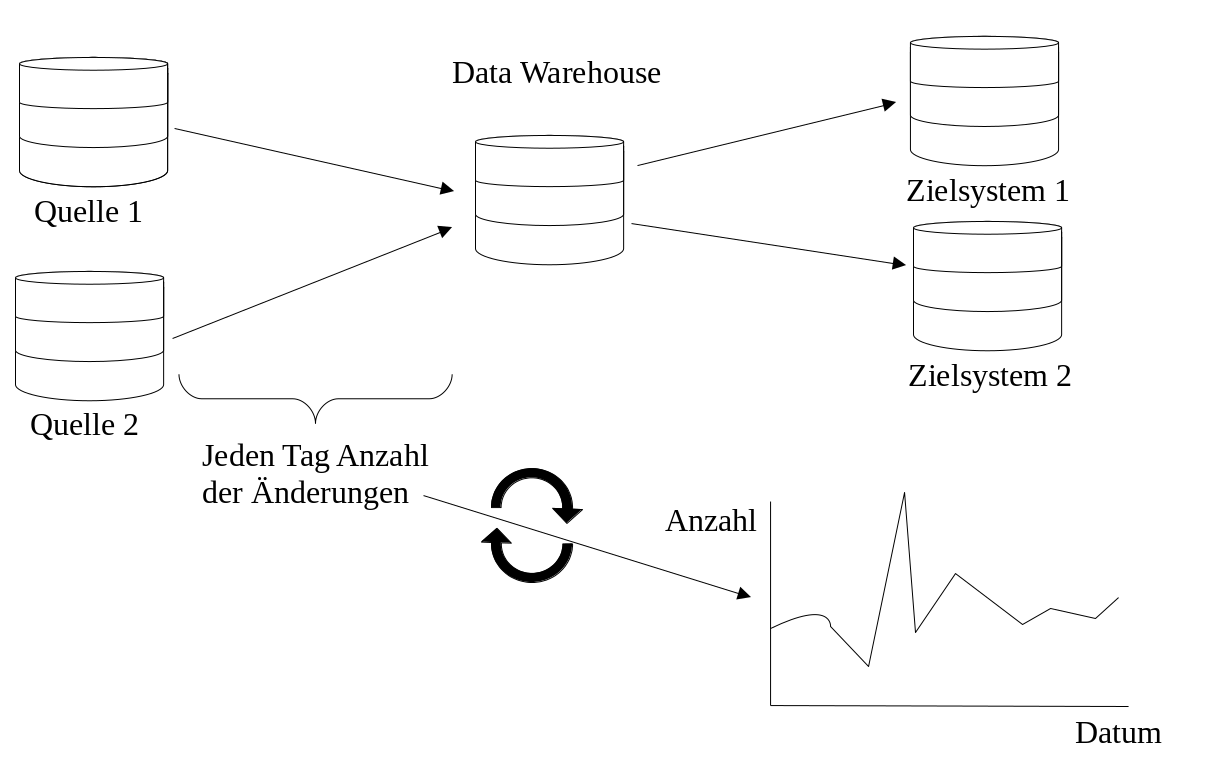
\includegraphics[width=150mm,scale=1]{content/Darstellung_vis_pipeline.png}
\caption{Darstellung des aktuellen Extraktionsverfahrens und Integration der Visualisierung }%
\end{figure}
Die Abbildung zeigt den aktuellen Extraktions-Prozess des Data Warehouse. 
Bei diesem werden Daten aus einigen Quellsystemen abgeholt und in eine zentrale Datenbank, dem Data Warehouse extrahiert.
Anschließend werden die Daten in das korrekte Format konvertiert und den Endsystemen so bereitgestellt, wie diese die Daten erwarten.

Eine mögliche Visualisierung sollte die Meta-Daten, die von den Quellsystemen extrahiert werden erhalten und anschließend visualisieren.
Hierfür wird per Trigger die Daten in Echtzeit an Elastic übertragen, dass die Daten anschließend mit Hilfe eines Kibana Dashboards visualisiert.
Stakeholder sind dann in der Lage grafisch zu sehen, ob es große Abweichungen zu den Monaten / Wochen / Jahren davor gegeben hat und können so einschätzen, ob genauer nachgeforscht werden muss oder ob alles geklappt hat.




%Daten zur Beladung (Delta, Vollbestand) in Echtzeit aus dem DWH nach Elastic exportieren
%-> Anhand eines Dashboards ist es möglich festzustellen, ob es Abweichungen gibt
%-> Ein Experte kann diese Abweichungen dann überprüfen



%Vollständigkeit auf Datensatzebene
%Vollständigkeit auf Attributwerte (es kommen keine null-values hinzu)


%Aktualität die Daten werden schnell genug abgeholt
%Richtigkeit die Daten werden so abgeholt, dass sie fehlerfrei sind

%Ideen:
%- Source und Target vergleichen
%- historisch vergleichen, wie viel zu erwarten ist
%- 

%Die Daten müssen innerhalb einer vorgelegten Range liegen, damit sichergestellt wird, dass die Daten in dem Zielsystem richtig ankommen.



%Zuverlässigkeit, Protokollierung, Dokumentation, Audit der Prozesse
% Verfügbarkeit, Wartbarkeit, Nachvollziehbarkeit








\chapter{Experimente}\label{ch:experiments}
%Auf Validität und Reliabilität achten!
Die ML-Experimente bestehen darin die Methoden praktisch umzusetzen und die Ergebnisse zu interpretieren. 
Ziel der Experimente ist einen Klassifikator zu trainieren, der den Risikoscore zuverlässig vorhersagen kann. 
Mit dessen Hilfe ist es anschließend möglich die Aktualität bzw. Richtigkeit des Scores zu überprüfen und zu aktualisieren.
Dies spart Geld, da nun nur noch die Daten aktualisiert werden müssen, bei denen der Klassifikator eine Abweichung feststellt. 
Auch für neue Kunden kann dieses Verfahren verwendet werden, um schnell ein Ergebnis zu erhalten, da nicht erst auf das Ergebnis der externen Ratingfirma gewartet werden muss.
Allerdings sollten die Daten immer aktualisiert werden und nicht nur auf den Klassifikator vertraut werden. 
Um die Datenmenge zu reduzieren, werden zunächst nur die Daten von einem bestimmten Tag geladen und analysiert.
Da die Klassifikatoren keine guten Ergebnisse aufweisen, wird als Lösung ein Upsampling der Daten vorgeschlagen, das die Lücken der Labels aus älteren Daten füllt.


\section{ML-Experimente / Modell Evaluation }

\subsection{Versuchsaufbau}
Die Experimente werden auf einem Windows-Rechner in einem Jupyter-Notebook durchgeführt.
Ein Jupyter Notebook ist ein interaktives Notizbuch, in dem Pythoncode geschrieben und ausgeführt werden kann.
Visualisierungen, wie Grafiken oder Plots von mathematischen Funktionen können direkt im Dokument betrachtet werden. 
Die Vorteile liegen darin, dass verschiedene Hypothesen einfach umgesetzt und getestet werden können. 
Dies ist auch für diese Experimente sinnvoll, da unterschiedliche Parameter bzw. Ansätze getestet werden.
Das hilft dabei festzustellen, welches Verfahren mit welchen Parametern am besten eignet ist, um Daten vorherzusagen. 

%Vorteile von Jupyter Notebook
Als Python-Bibliotheken kommen pandas, numpy und sklearn zum Einsatz. 
\\
Vorgehensweise: \\


Zunächst werden die Daten mit Hilfe eines Python-Connectors von der Datenbank in das Jupyter Notebook geladen, die wie im Kapitel 3 beschrieben, durch ein Skript erzeugt werden.
%Code Exzerpt: 
Hierfür werden die Daten in ein Python-Dictionary geladen und anschließend in einer Python-Tabelle (DataFrame) gespeichert. 
Dies geschieht mit Hilfe des IBM DB2-Connectors. 
Dieses Framework ermöglicht es die Daten mit Hilfe eines SQL-Befehls direkt von der Datenbank zu extrahieren.
Deshalb können die Daten für die Experimente mit SQL von der Datenbank vorbereitet werden.%Under oversampling, train test aufteilung
Das hat den Vorteil, dass die Daten von einem Datenbankserver vorverarbeitet werden, der direkten Zugriff auf die Daten hat.
Deshalb müssen weniger Daten über das Netzwerk übertragen werden, wenn die Daten durch ein SQL eingeschränkt werden und nicht erst aus dem DataFrame in Python entfernt werden müssen. 

% was ist ein Python-Dictionary und ein DataFrame 

\subsection{Untersuchung von textuellen Daten}
In \autoref{sec:textVerfahren} werden die Möglichkeiten zur Verwendung von Rechtschreibprüfungen zur Untersuchung von Datenqualität dargestellt und erläutert.
Hierfür werden nachfolgend die Verfahren anhand des Programmcodes erläutert und beispielhaft für die Datenspalte 'Berufe' durchgeführt. 
Die Ergebnisse werden auch in dem nachfolgend beschriebenem Dashboard angezeigt, indem die Daten in einer MySQL-Datenbank gespeichert und anschließend visualisiert werden. 


Zunächst muss für die deutsche Sprache ein Wörterbuch installiert werden. 
Auf einem Linux-Rechner kann dies mit dem Befehl 'sudo apt-get install myspell-de' nachinstalliert werden. 
Für Windows muss zunächst der Ordner gefunden werden, in dem die Daten vom python-Paketmanager gespeichert werden. \cite{https://pyenchant.github.io/pyenchant/install.html}
Mit dem Python-Code 'import enchant print(enchant.Broker().describe()' kann herausgefunden werden, welche Implementierung verwendet wird, um die Rechtschreibprüfung durchzuführen.
Diese Information ist notwendig, um den korrekten Ordner in der Python-Installation zu finden. 
Für die deutsche Sprache kann das Wörterbuch igerman98 \cite{https://www.j3e.de/ispell/igerman98/} verwendet werden. %-- TODO unter gnu gpl v3 lizensiert

Um das Textfeld der Berufe zu analysieren werden diese zunächst mit dem Paket numpy, das für numerische Verfahren in python verwendet wird, aggregiert.
Dies hat den Vorteil, dass gleiche Wörter einmalig von der Rechtschreibprüfung analysiert werden müssen. 
Da es sich bei den Textdaten um Berufe handelt und es nur eine begrenzte Anzahl von unterschiedlichen Berufen gibt ist davon auszugehen, dass sich einige der Daten überschneiden. 
Der nachfolgende Programmcode zeigt die Verwendung der Funktion unique in numpy und die Konvertierung in einen Python DataFrame, der zur Weiterverarbeitung verwendet wird, vgl. \cite{https://numpy.org/doc/stable/reference/generated/numpy.unique.html}. \\


\begin{minipage}{\linewidth}
\begin{lstlisting}[language=Python,caption={Extraktion der eindeutigen Texte},captionpos=b]
 import numpy as np 
 unique, counts = np.unique(df['BERUF'], return_counts=True)
 df = pd.DataFrame(zip(unique, counts))
\end{lstlisting}
\end{minipage}


Anschließend wird die Rechtschreibprüfung auf alle einzigartigen Ausprägungen der Berufsbezeichnung angewendet und die Anzahl der Werte addiert. 
Hierfür wird zunächst das für die Sprache korrekte Wörterbuch ausgewählt. 
Um den Fortschritt der Ausführung sehen zu können, wird die Python Bibliothek tqdm %TODO bib beschreiben
verwendet. 
Anschließend wird durch die Verwendung des SpellCheckers, der in pyenchant enthalten ist, jedes Wort geprüft und im Fehlerfall auf den Zähler addiert.
Die Implementierung des beschriebenen Szenarios ist in nachfolgendem Listing zu erkennen. 
Insbesondere ist die Umsetzung der Verwendung des SpellCheckers in den Zeilen 8, 9 und 10 zu sehen. 

\begin{minipage}{\linewidth}
\begin{lstlisting}[language=Python,caption={Implementierung der Rechtschreibprüfung},captionpos=b]
 import enchant
 from tqdm import tqdm 
 from enchant.checker import SpellChecker
 
 spellChecker = SpellChecker(enchant.Dict("de_DE"))
 counter = 0
 
 for idx, row in tqdm(df.iterrows(), total=df.shape[0]):
    spellChecker.set_text(row[0])
    for err in spellChecker: 
        counter+=row[1]
\end{lstlisting}
\end{minipage}

Um den Netzwerkverkehr zu reduzieren werden nur die Daten in den DataFrame geladen, die eine Berufsbezeichnung beinhalten. 
Zur Berechnung der Gesamtzahl der verfügbaren Berufe werden mit Hilfe eines SQL Counts die Anzahl der Daten berechnet.
Der Anteil der Daten mit Rechtschreibfehler, kann durch eine Division der Wörter mit Rechtschreibfehler und der Gesamtzahl aller Wörter berechnet werden und liegt bei knapp 24\%. 


Das Ergebnis dieser Berechnung muss nun für die Visualisierung in einer Datenbank gespeichert werden, damit diese darauf zugreifen kann. 
Hierfür wird ein Python Skript verwendet, das die Berechnung durchführt und anschließend mit einem SQL Insert in der Datenbank speichert. 
Das Python Skript kann entweder mit Hilfe eines Cron Jobs einmal pro Nacht ausgeführt oder in die Jobsteuerung des DataWarehouse integriert werden.


Es sind in den berechneten 24\% fehlerbehafteten Daten auch Fehler enthalten, die darauf zurückzuführen sind, dass die Rechtschreibprüfung Abkürzungen wie z. B. 'techn' oder 'öfftl' nicht kennt. 
Allerdings ist es sinnvoll diese auch auszubessern, um eine bessere Datenqualität zu erreichen.
Dafür gibt es mehrere Gründe, warum dies zu einer besseren Datenqualität führt.
Zum einen kann es zu Mehrdeutigkeiten von Abkürzungen kommen, die zu Fehlern führen, weil die wahre Bedeutung unterschiedlich interpretiert werden kann. 
Zum anderen können für das gleiche Wort mehrere Abkürzungen verwendet werden, wie z. B. 'öff.', 'öfftl.', 'öffentl.'.
Wenn für die gleiche Bedeutung eines Wortes mehrere Abkürzungen vorhanden sind, ist es schwieriger diese auszuwerten.
Möchte man alle Personen, die im öffentlichen Dienst arbeiten aus den Daten extrahieren, so müsste man in diesem Datensatz alle denkbaren Abkürzungen bei der Abfrage mit angeben. 




\subsection{Erzeugen der ABT und Erstellen eines Data Quality Reports}

\subsection{Datenaufbereitung }
Zunächst werden die Daten genauer untersucht, um festzustellen ob die Daten bereinigt werden müssen oder ob sich die Klassenverteilung zu sehr unterscheidet. 
Zunächst zeigt eine Grafik die Verteilung der einzelnen Klassen. 
In der Abbildung ist zu erkennen, dass die Klassen sehr ungleichmäßig verteilt sind.

Klasse 0E ist deutlich häufiger vertreten als die anderen Klassen. 
Dies führt für einige Verfahren zu Problemen und sollte behoben und vor allem durch die Verwendung von geeigneten Metriken beobachtet werden.


%---------------------- Todo EVTL in neues Kapitel verschieben 
Außerdem sind in dem vorliegen Datensatz einige textuelle Attribute.
Diese können durch einen OneHot Encoder so aufbereitet werden, dass sie in einem Klassifikator verwendet werden können.
Das Feld 'BERUF' besteht aus Berufen, die von den Bankmitarbeitern eingetragen werden.
Da die Berufsbezeichnung nicht genderneutral notiert sind, wird mit Hilfe eines Stemmings die Daten auf eine gemeinsame Grundform überführt.
Hierbei wird der Snowball Stemmer von NLTK verwendet, da dieser auch für die Deutsche Sprache geeignet ist.
%----------------------

Nach einem OneHot Encoding entstehen viele Nullen in dem Datenset.
Deshalb bietet sich zur weiteren Verarbeitung eine Sparse-Matrix an.
Diese speichert nur die tatsächlich vorhandenen Daten und speichert keine Null-Werte. %Quelle

Da manche Daten sehr von anderen abweichen (Varianz sehr groß) müssen die Daten skaliert werden.
Zum Beispiel kann der Saldo einen Wertebereich von [-100.000;100.000] haben.
Die Standardabweichung ist sehr groß, da die Daten einen großen Wertebereich haben.
Aus der Formel zur Berechnung der Standardabweichung ergibt sich somit folgende Tabelle:

      | Werte bereich,      | Standardabweichung
SALDO | -100.000, 100.000   | 100.000

%Varianz ausrechnen und als Tabellenausschnitt anzeigen

Des weiteren können Daten entfernt werden, die nur einen einzigen Wert haben, da diese keinen Klassifikator trainieren können.



\subsection{Machine Learning}
\label{sub:machine_learning}
Die verwendeten Verfahren beruhen auf den in Kapitel 4 ausgewählten Methoden.
Anhand der nachfolgenden Experimente und der genauen Analyse der Daten ist zu Erkennen, dass die Klassenverteilung sehr unausgeglichen ist. 
Dies hat zur Folge, dass die gewählten Modelle zum einen nicht richtig trainiert und zum anderen nicht korrekt validiert werden können. 
Es ist deshalb wichtig die korrekten Verfahren zur Modellbewertung zu beachten.
Das heißt konkret, dass außer dem Accuracy-Score auch andere Metriken betrachtet werden müssen, wie z.B. Precision und Recall.


\textbf{Warum Undersampling?}
% Eine Baseline stellt ein einfaches Modell dar, das versucht wird zu verbessern. 
Als Beispiel zum Problem der ungleichen Klassenverteilung soll folgendes Szenario zeigen: \\
Die Klassenverteilung der Daten zeigt, dass die Klasse '0E' einen Anteil von knapp 58\% besitzen. 
Ein einfacher Klassifikator, der immer diese Klasse rät, würde somit eine Accurracy von 58\% erreichen. % TODO  \textbf{HIER NOCH DIE FORMEL EINFÜGEN}
Da Undersampling generell zu weniger Over-Fitting führt als oversampling wird zunächst versucht dieses Verfahren zu verwenden. \cite{fundamentals of ml}
%In der Liste der Klassen ist die Klasse '4A' nicht so häufig vertreten, weshalb eine Kombination der beiden Verfahren nachfolgend getestet wird. 
Das Undersampling sollte jedoch nur auf den Trainigsdaten erfolgen und nicht bevor die Daten in Trainings- und Testset extrahiert werden, da sonst die Gefahr besteht, dass das Modell nicht korrekt in der realen Verwendung funktioniert. 

% WIRD JETZT ANDERS GEMACHT Da die Daten nicht in den Arbeitsspeicher des Entwicklungsrechners passen wird die Funktionalität des Train / Testsplit zunächst in SQL geschrieben, damit dies von dem Datenbankserver übernommen werden kann, der genügend Ressourcen zur Verfügung hat. 



\textbf{Aufteilen in train/validation/test}
Um ein Overfitting zu vermeiden und auch erkennen zu können bietet sich die Aufteilung der Daten in drei Kategorien an.
Der größte Anteil wird für das Training verwendet.
Zusätzlich zu einem test-Datensatz wird allerdings noch ein Validierungs-Datensatz extrahiert.
Dieser Datensatz wird während der Parameteranpassung nicht verwendet und so kann anhand diesen Datensatzes erkannt werden, wie gut sich das Modell bei neuen, ungesehenen Daten verhalten würde. 
Typische Größen zur Aufteilung liegen bei 50:20:30 oder 40:20:40. 
In diesem Projekt wird der Split bei 50:20:30 gesetzt, um einen möglichst großen Anteil an Daten für das Training zur Verfügung zu haben. 
\cite{Fundamentals of ML Kapitel 8}
In konkreten Zahlen bedeutet das eine Aufteilung in 60.000, 24.000 und 36.000. 
%67.257, 26903, 40354
Da die Daten zur Validierung nicht während des 

%Jedes Verfahren wird mit Upsampling brauchbar gemacht.
%Warum? (grob: was ist upsampling / oder Kapitel 4 verweisen)
%Wie wird das Upsampling gemacht?

\textbf{Erstellen einer Baseline}
https://datascience.stackexchange.com/questions/30912/what-does-baseline-mean-in-the-context-of-machine-learning

Zunächst wird für die Durchführung der Machine Learning Experimente ein Modell erzeugt, dass auf eine primitive Weise das Problem löst.
Dadurch kann mit einem Ansatz verglichen werden und in den Experimenten ist erkennbar, ob die neu gewählten Modelle besser als der naive Ansatz sind. %\cite{https://developers.google.com/machine-learning/glossary#baseline}
Ziel ist es einen Klassifikator zu definieren, der besser als das einfache Modell ist. 
Ein baseline Ergebnis bezeichnet die einfachste mögliche Vorhersage. 
Bei einem Klassifikationsproblem kann beispielsweise als Vorhersage immer die am häufigsten vertretene Klasse verwendet werden. \cite{brownlee2014}
Mit Hilfe einer Baseline kann durch Vergleiche herausgefunden werden, ob die Verwendung von anderen Attributen oder einem anderen Klassifikator bessere Ergebnisse liefern. \cite{brownlee2014}

Ein Baseline Modell kann mit Hilfe des DummyClassifiers von sklearn erzeugt werden. 
Dieses kann mit Hilfe von verschiedenen Strategien ein einfaches Modell definieren und dessen Performance getestet werden. %siehe https://scikit-learn.org/stable/modules/model_evaluation.html#dummy-estimators

Es werden verschiedene Baseline Modelle getestet und das beste für die weiteren Vergleiche verwendet. 
Dieses wird mit dem Parameter 'most\_frequent' erreicht und hat eine Accuracy von 55\% und eine Precision von 31\%. 

\textbf{Ergebnisse aus den vorgestellten Verfahren}
Für die einzelnen Klassifikatoren, die in \autoref{ch:methods} definiert und beschrieben sind, werden die Experimente nachfolgend durchgeführt.
Hierfür werden die Parameter angepasst, die die Klassifikatoren definieren. %Evtl wird hier auch mit RandomizedSearchCV getestet
Des weiteren werden Datenverbesserungen, wie Scaling und das Entfernen von Outliers getestet. 
Die Ergebnisse werden nachfolgend aufgelistet und das beste der Ergebnisse abschließend beschrieben. 
Als Vergleich soll das Baseline Modell dienen, das im vorherigen Abschnitt definiert ist.



\begin{tabular}[h]{l|c|c|c}
Klassifikator & Accuracy        & Precision & Scaler \\ \hline
Baseline & 0.55 & 0.31 & Standard Scaler \\
KNN & 0.583 & 0.464 & Standard Scaler \\
RandomForest & 0.544 & 0.55 & Standard Scaler \\


Baseline & 0.55 & 0.30 & Kein Scaler \\
KNN & 0.565 & 0.43 & Kein Scaler \\
Random Forest & 0.63 & 0.57 & Kein Scaler \\

\end{tabular}




KNN
- trainieren
    - Mit / Ohne Upsampling
    - Mit gleicher / ungleicher Klassenverteilung
    - unterschiedliche K - Werte
- Modell Bewerten 
    - train dev test
    - f1-score, accuracy und precision
    - stratified k-fold cross validation
    - f1-score, accuracy und precision 

    
SVM
- trainieren
- Modell Bewerten 
    - train dev test
    - f1-score, accuracy und precision
    - stratified k-fold cross validation
    - f1-score, accuracy und precision 

Random Forest
- trainieren
- Modell Bewerten 
    - train dev test
    - f1-score, accuracy und precision
    - stratified k-fold cross validation
    - f1-score, accuracy und precision 


Zusammenfassung: Welcher hat das beste Klassifikationsergebnis?
In diesem Kapitel wurden die Verfahren KNN, SVM, blabla getestet und der beste Klassifikator ist blabla.

\subsection{Evaluation der Machine Learning Modelle}
\label{sub:evaluation}



%Scoringverfahren:



%Was sind Daten die Einfluss auf das Kundenrating haben?
%-> Für welche Daten wäre es besonders wichtig die Datenqualität händisch zu überprüfen


%ML-Verfahren, immer inklusive Performance-Grafik:
%- logistische Regression


%Ziele:
%- Vorhersagen des Risikoscorings anhand der Inputdaten

%Aufbau:
%- python als Programmiersprache
%- Aufteilen in train-dev-test
%- 


%\subsection{KNN}

%Variabilität (Einfluss der Parameter auf das Ergebnis):
%- verschiedene k-Werte 
%- Manhattan vs. Euklidische Distanz


%\subsection{SVM (Multiklassen)}

%Verschiedene Parameter:
%- unterschiedl. Kernelfunktionen
%- C-Parameter, der über Slackvariablen gesteuert wird
%- 

%- Neuronale Netze

%- Classifikation Tree



%Aufbau Experimente: 
%Ziele*ʹ Aufbau*ʹ Ergebnisse*' Interpretation*ʹ Threats*to*Validity
%(Seite 93 https://userpages.uni-koblenz.de/~laemmel/esecourse/slides/perf.pdf)


%Ideen:
%- Komplexe Funktionen mit Stakeholdern basteln, zb wenn verheiratet dann Alter > 18
%- Daten für zb Aktualität müssen definiert werden, ob sie beispielsweise überhaupt verfallen können. Zb Geburtsdatum ändert sich nie; Alter schon
%- Ist es möglich solche Regeln mit HIlfe von ML abzuleiten oder funktioniert das gar nicht? 
%- Daten vor einem Monat berechnen, wie viele sich ändern müssten (aufgrund von zb Timeliness, correctness) und dann nachschauen wie viele sich tatsächlich geändert haben
%- Big Data Quality A Quality Dimension evaluation hat zwei konkrete Experimente, dort kann man sich gute Ideen holen. Es wird auch ein Experte zu Rate gezogen, der beispielsweise angibt, welche Daten gelöscht werden können (zb wenn 80\% der Attribute fehlen). Es hat auch einige Visualisierungen 
%- Mit SQL: 
%https://dataform.co/blog/advanced-data-quality-testing




%Auf die verschiedenen Ebenen Aktualität, Richtigkeit, Vollständigkeit und Konsistenz eingehen!
%Oft ist es besser die Daten nachzufordern, anhand eines möglichen Fehlers kann nicht der Originalzustand wiederhergestellt werden

%\section{Visualisierung}

%https://www.elastic.co/guide/en/kibana/6.8/createvis.html

\subsection{Visualisierung}
\label{sub:visualisierung}
Damit die Daten für die Visualisierung verfügbar sind, müssen diese zunächst in das Visualisierungstool integriert werden. 
Da zur Erstellung des Dashboards das Tool Grafana vorgeschlagen und verwendet wird, müssen die Daten an Grafana angebunden werden.

Wie bereits erwähnt, ist es zwar sinnvoll einen Konnektor zu verwenden, allerdings gibt es keinen Konnektor zwischen Grafana und der DB2 Datenbank.  \\

Folgende Lösung zur Integration der Daten wird im Projekt stattdessen verwendet. 
Die Daten werden mit Hilfe der DB2-Exportfunktionalität exportiert und als CSV-Datei gespeichert. 
Diese Datei wird anschließend mit Hilfe von SQL in eine MySQL Datenbank exportiert. 
Um die Daten regelmäßig zu migrieren kann ein Cron-Job verwendet werden, der beispielsweise einmal in der Nacht ausgeführt wird. 
In Zukunft kann das ETL-Tool, mit dem die Daten aus den Quellsystemen gesammelt und aggregiert werden, verwendet werden, um die Daten direkt in die MySQL Datenbank zu exportieren.
Da dieses Tool eine Steuerung zur automatischen Ausführung von Programmen beinhaltet ist es möglich den Export dort zu hinterlegen und es ist kein Cron-Job mehr nötig. 

%Verweis auf Grafana Kapitel



\textbf{Untersuchung der Dimension Richtigkeit} \\
Anhand der Analyse der Daten in einer Zeitreihe, kann erkannt werden, ob in bestimmten Zeiträumen auffällig viele bzw. wenige Datensätze vorhanden sind. 
Mit Hilfe der Visualisierung lassen sich auffällige Tage erkennen, die nicht dem Muster entsprechen. 
Dabei ist allerdings nur auf einer abstrakteren Ebene zu erkennen, ob es ein Problem in der Datenverarbeitung gegeben hat. 
Beispielsweise ist nicht zu erkennen, ob sich eine Datenreihe von einem konkreten Konto besonders auffällig verändert hat, da diese Analysen in dieser gruppierten Darstellung untergehen. 

Zunächst werden für eine Untersuchung die Daten jeweils nach dem aktuell gültigem Datum gruppiert und der aktuelle Saldo summiert.
Dies wird als SQL-Befehl in Grafana in einem neuen Dashboard bzw. Panel hinterlegt.
An der rechten Seite kann die Visualisierung ausgewählt und farblich angepasst werden.
Des weiteren muss der richtige Zeitraum ausgewählt werden, sodass die Daten angezeigt werden können.

\begin{figure}[h]
\centering
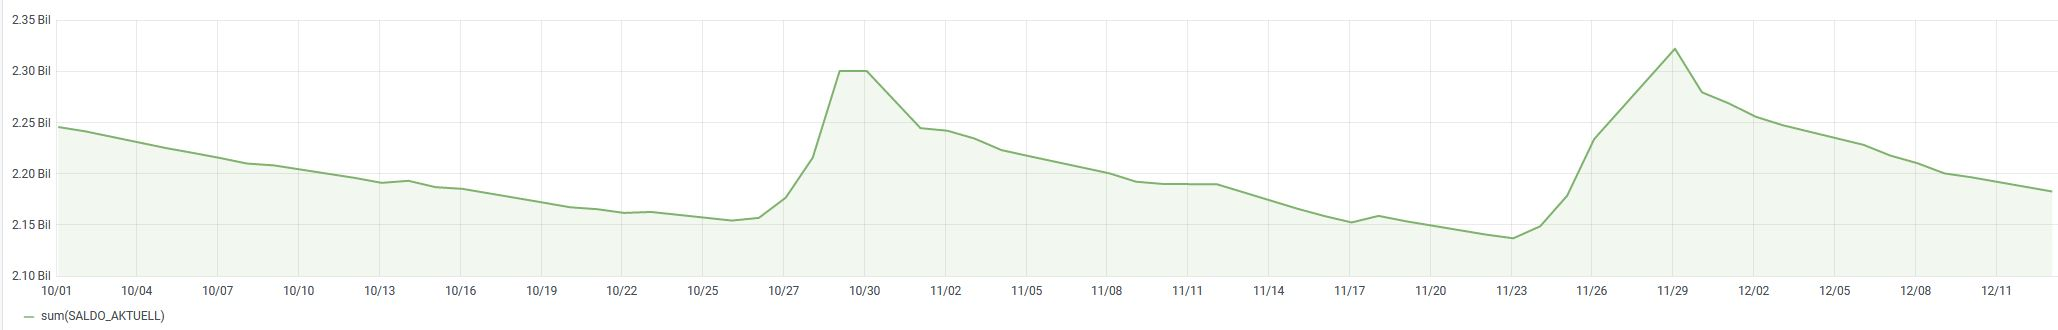
\includegraphics[width=150mm,scale=1]{content/Saldo_aktuell.jpg}
\caption{Visualisierung der Veränderung des Saldos}%
\end{figure}


In der Grafik ist ein eindeutiges Muster zu erkennen. 
Bei der Analyse von drei Monaten ist zu sehen, dass immer zum Ende bzw. Anfang des neuen Monats der Gesamtsaldo aller Konten besonders hoch ist. 
Dies ist vermutlich damit zu erklären, dass am Anfang des Monats viele Personen ihr Gehalt erhalten und somit das Gesamtsaldo aller Konten zu diesem Zeitpunkt steigt. 
Für einen Stakeholder ist diese Information und Art der Überwachung interessant, da dieser in der Lage ist zu überprüfen, ob es Probleme mit den Prozessen zur Extraktion der Daten gegeben hat. 
Die Datenwerte sollten immer diese monatlichen Schwankungen aufweisen.
Sobald diese nicht mehr auftreten, deutet das auf ein Problem hin, das von den Stakeholdern genauer untersucht werden sollte. 
Dieses Verfahren kann von den Entwickler verwendet werden, um sie dabei zu unterstützen ihre Arbeitsergebnisse zu überprüfen.



\begin{figure}[h]
\centering
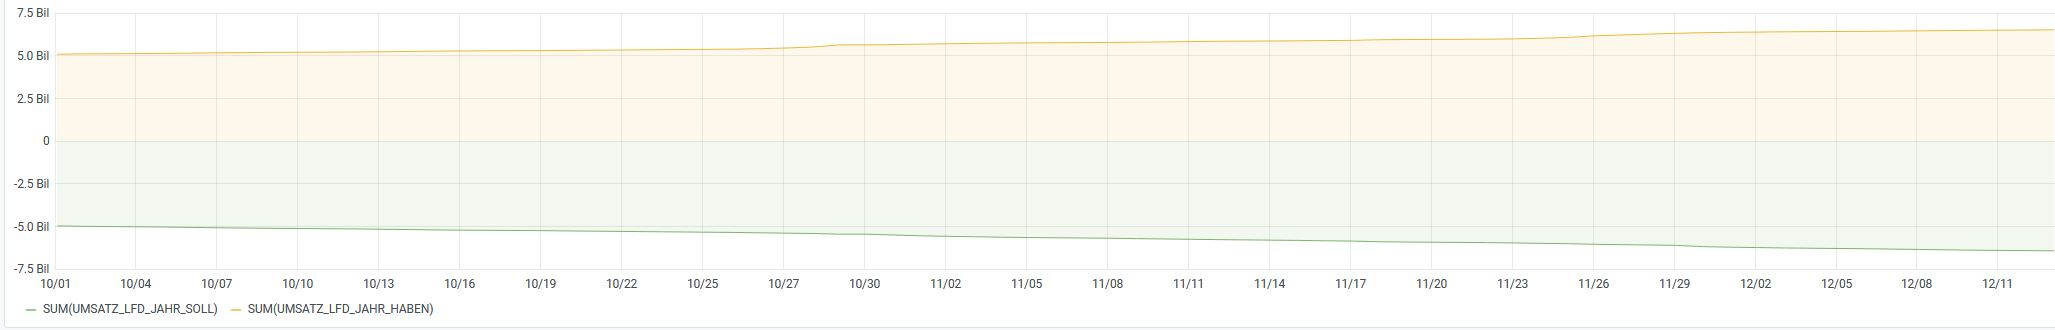
\includegraphics[width=150mm,scale=1]{content/vergleich_haben_soll.jpg}
\caption{Vergleich von Haben und Soll Umsatz}%
\end{figure}

In der Grafik ist zu erkennen, dass die Summe des Umsatzes zum Ende des Jahres generell steigen. 
Des weiteren zeigt die Datenreihe das Verhältnis des Umsatzsolls, welcher anzeigt, wie viel ausgegeben wurde. 
Da die meisten deutschen Bürger so wirtschaften, dass sie am Ende vom Jahr immer auf einen leichten Plus kommen ist zu erwarten, dass die Menge der Ausgaben insgesamt ungefähr gleich der Einnahmen ist. \cite{https://www.welt.de/wirtschaft/article189283761/Sparverhalten-der-Deutschen-Fast-jeder-Dritte-hat-am-Monatsende-kein-Geld-mehr.html}
Auch dieses Phänomen ist in der erstellten Grafik zu erkennen. 
Der negative Wert stellt den Umsatzsoll dar, dieser ist orange gekennzeichnet. 
Als Gegenpol ist in der Grafik der Umsatzhaben aufgetragen. 
Insgesamt müssen die beiden Linien sich ungefähr ergänzen. 


\textbf{Untersuchung der Dimension Vollständigkeit} \\
Um den Stakeholdern eine Möglichkeit zu geben, zu erkennen wie viele der Daten befüllt sind, bietet sich die Dimension der Vollständigkeit an.
Diese gibt an, wie viel Prozent der Datenwerte einen Wert beinhalten, also nicht null oder leer sind. 
Im vorliegenden Beispiel werden für das Dashboard die Anzahl der Kunden berechnet, die keine Berufsbezeichnung haben. 
Hierfür wird mit Hilfe eines SQLs die Gesamtzahl aller Daten, sowie der Anzahl der Daten ohne Berufsbezeichnung berechnet und anschließend geteilt. 
Einige der Daten besitzen keine Auskunft über den Beruf der Person. 
Sinnvoll wäre hier allerdings den Wert auf arbeitslos zu setzen, bei den Personen, die tatsächlich keinen Beruf haben. 
Dadurch werden die Missverständnisse aufgelöst, die entstehen, wenn eine Person als arbeitlos gewertet wird, obwohl sie einfach nur keinen Beruf angegeben hat. 
Man kann hier nicht davon ausgehen, dass die Personen keinen Beruf haben, sondern nur, dass die Daten nicht vollständig sind.









%Weitere werte die visualisiert werden, zb Anzahl der Kunden


\textbf{finden von besonders auffälligen Punkten}




\section{Diskussion zu den Dashboards}
%evtl. verschieben in ein Chapter, oder zwei mal verwenden, einmal bei Visualisierung und einmal bei ML Verfahren 
Anhand des erstellten Dashboards können die Entwickler sofort erkennen, ob durch ihre Programmänderungen, Fehler entstanden sind. 
Dies ist besonders hilfreich, da die Entwickler normalerweise nicht die gesamte Auswirkung ihrer Änderung sehen können. 
So kann die Änderung eines einzelnen Datenwertes zu Auswirkungen am Ende des Extraktionsprozesses führen, ohne dass diese direkt in der Tabelle erkannt werden, für die ein Programm angepasst wird.
Dies liegt daran, dass die Extraktionsprozesse sehr komplex sind und die Zusammenhänge der Daten nicht sofort ersichtlich sind. 
Für die Visualisierungen werden mehrere Tabellen benötigt, aus denen die Daten zusammengetragen (gejoint) werden, dadurch werden indirekt die Zusammenhänge zwischen den Daten aufgezeigt, da die Daten gesamthaft betrachtet werden. 

Auch während der Durchführung der Experimente konnte so ein Fehler entdeckt werden. 
Dieser ist dadurch aufgetreten, dass die Extraktion der Daten von DB2 als Trennzeichen ein Komma verwendet hat. 
Da die Zahlenwerte in deutscher Repräsentation abgespeichert und extrahiert werden, wird ein Komma als Dezimaltrennzeichen verwendet. 
Dieses Problem konnte erkannt werden, da die Daten des Soll-Umsatzes um ein Vielfaches von den Daten des Haben-Umsatzes abweichen. 
Die Lösung besteht darin ein anderes Trennzeichen der Datenwerte zu verwenden, das nicht in den anderen Daten vorhanden ist. 








- Data Quality Report anhand der ABT.


Integration der Daten in Kibana
- ETL Prozess zur automatischen Erzeugung einer CSV-Datei.
- Logstash?
- 

- Visualisierung von Unterschieden:
- Aggregiert nach Wochentag / Monat
- Umsatzdaten
- Kundendaten (Neukundenzuwachs?)


Kibana, Graphana

Reduktion der Datenmenge



- Welche Visualisierungen bieten sich an?
- Gibt es evtl. Visualisierungen, die DQ-Probleme aufzeigen?

\chapter{Ausblick}\label{ch:outlook}
%Nachfolgend alles Fazit: ?
Die Ergebnisse der Klassifikation sind nicht so gut, wie erwartet. 
Allerdings konnte gezeigt werden, dass es prinzipiell möglich ist Daten vorherzusagen.
Durch die Ausarbeitungen der Datenaufbereitung können zukünftig neue Experimente durchgeführt werden, ohne die Daten beschaffen zu müssen. 
Es ist somit sehr viel schneller möglich Experimente durchzuführen.
Deshalb ist für einen produktiven Einsatz wichtig den trainierten Klassifikator an den korrekten Positionen einzusetzen, um einen tatsächlichen Mehrwert zu schaffen.


%Ausblick
In weiteren Experimenten sollten noch weitere Klassifikatoren und deren Performance getestet werden.
Hierfür könnten sich Neuronale Netze anbieten, da diese gezeigt haben, dass sie für sehr viele verschiedene Anwendungsgebiete gute Ergebnisse erzielen.
Es sollten noch weitere Daten exportiert werden. 
Aktuell liegen Daten von knapp einem Jahr vor, allerdings können die Ergebnisse noch weiter verbessert werden, wenn noch mehr Daten von den Klassen, die sehr wenig vertreten sind, zum Training gesammelt werden. 

% Binning (Numerische Featues in kategorien einteilen erste 1000, nächste 1000 usw) Kapitel 3.6.2 Fundamental of ML

Um das Thema Datenqualität vollständig innerhalb eines Data Warehouse umzusetzen und zu etablieren sind noch einige weitere Schritte nötig.
Außer den vorgestellten Methoden zur automatischen Analyse und Visualisierung der Datenqualität, sind manuelle Tätigkeiten nötig.
Hierfür müssen die Business User 


Des Weiteren kann es sinnvoll sein sich mit unüberwachtem Lernen und Verfahren im Bezug auf Datenqualität zu beschäftigen.
Hierfür wurde in der Arbeit die Idee und der Ansatz von Talend skizziert. 
Allerdings benötigt dieses Verfahren manuelle Tätigkeiten und nutzt so nicht die Vorteile von automatischen und unüberwachten Lernmethoden aus. 





Textuelle Daten: 
% TODO Als Erweiterung kann der SpellChecker verwendet werden, um direkt die Daten zu verbessern, in dem dieser verwendet wird und die besten passenden Wörter als Alternative einsetzt. 
% Dies ist allerdings mit Vorsicht zu benutzen, da so gravierendere Fehler entstehen können, wenn der SpellChecker Wörter als richtig ansieht, die nichts mit dem eigentlichen Wort zu tun haben. 
% Vor allem liegt dies daran, dass der SpellChecker keine inoffiziellen Abkürzungen kennt. 
% Beispielsweise schlägt der Spellchecker für die Abkürzung 'öfftl', die vermutlich öffentlich bedeuten soll, das Wort Löffel vor. 
Grafana:
In dem Projekt wird aus einfachheitsgründen MySQL benutzt
Zukünftig könnte bzw sollte hier eine Influxdb oder graphite zum einsatz kommen, da diese Time Series Datenbanken sind und perfekt für die Anfragen geeignet sind

Visualisierung:
Weitere Dashboards. Mehr Daten sammeln. Zukünftige Beobachtungen nachvollziehen. 



In einer zukünftigen Version des Dashboards könnten die Tickets, die die Lösung des Problems beinhalten verknüpft werden. 
So kann ein Entscheider sofort erkennen, wie weit die Lösung des Problems ist und ob überhaupt eine Lösung des Problems beauftragt wurde. 
Dafür kann das für Grafana verfügbare Plugin 'Jira' verwendet werden. \cite{https://grafana.com/grafana/plugins/grafana-jira-datasource?pg=plugins&plcmt=featured-undefined}
Zusätzlich zur Anbindung von Jira als Ticketservice für Entwicklungstickets, könnte ServiceNow angebunden werden, um auch technische Probleme der Server oder der Infrastruktur zu überwachen. 
\cite{https://grafana.com/grafana/plugins/grafana-servicenow-datasource?pg=plugins&plcmt=featured-undefined}
Durch das Anbinden dieser Datenquelle ist es für einen Entscheider einfacher zu erkennen, ob das Problem, der schlechteren Datenqualität, durch die Entwicklungs- oder Infrastrukturabteilung entstanden ist. 
Anhand dieser Verknüpfung kann auch erkannt werden, welche der Tickets für das Auftreten eines Datenqualitätsproblems verantwortlich sein könnte, indem die Bearbeitungs- bzw. Fertigstellzeit mit dem Auftreten des Problems verglichen wird. 


\chapter{Fazit}\label{ch:summary}

Datenqualität ist unsichtbar, wenn alles richtig gemacht wird.

Es ist schwer zum Thema Datenqualität konkrete Lösungen bzw. Anwendungsfälle zu finden, da die meisten Arbeiten nur auf einem theoretischem Niveau unterwegs sind.
Auch große Beratungsfirmen zeigen nur Schritte auf, wie es theoretisch möglich ist, die Datenqualität zu Monitoren und zu verbessern.

Diese Arbeit zeigt exemplarisch für einen konkreten Fall, wie für diesen die Datenqualität im Bezug auf Aktualität analysiert und auch verbessert werden kann.

Allerdings ist es nicht für alle Problemfelder möglich mit automatischen Verfahren zu arbeiten, sondern es ist das Wissen von Businessusern bzw. Stakeholdern nötig, die konkrete Zielwerte vorgeben, um die Datenqualität zu überprüfen.
Hierfür sollten außer den vorgestellten Methoden noch manuelle Verfahren etabliert werden, die überprüfen, ob bestimmte Zielwerte eingehalten werden. 
Dafür sind umfangreiche Aussagen über die Daten nötig, wie z. B. Schwellwerte. 
Die benötigten Metadaten müssten zunächst von Experten festgelegt werden.

Des weiteren könnte ein Datensatz hilfreich sein, der konkrete Labels für gute bzw. schlechte Datenqualität besitzt. 
Dies könnte erreicht werden, indem Änderungen am Datensatz nur mit einer Begründung erfolgen kann.
Der Bearbeiter, der den Datensatz ändert, müsste so hinterlegen, warum der Datensatz aktualisiert worden ist. 

Da dieser Datensatz nicht existiert, musste damit gearbeitet werden, was vorhanden ist.


% remove if not needed
\appendix
\input{content/a1_supplemental}

\backmatter
\listoffigures
\cleardoublepage

\listoftables
\cleardoublepage

\renewcommand{\lstlistlistingname}{Auflistung}  % change for German thesis
\lstlistoflistings
\cleardoublepage

%TODO auf ieetr ändern? 
\bibliographystyle{wmaainf}
\bibliography{refs}

\printnoidxglossaries

\end{document}
